\documentclass[oneside,11pt,dvipsnames]{book}

\usepackage[utf8]{inputenc}
\usepackage[T1]{fontenc}
\usepackage[margin=1.5in]{geometry}
\usepackage{amsmath,amssymb,amsthm}
\usepackage{soul}
% \usepackage[small,compact]{titlesec} %very powerful
\usepackage[most]{tcolorbox}
% \setsecnumdepth{subsection}
% \setcounter{tocdepth}{3}
\usepackage{multirow,multicol}
\usepackage{enumitem}
\usepackage{epigraph}
\usepackage{cite}
\usepackage{caption}
\captionsetup{font=small}
\usepackage{graphicx}
\usepackage{pdfpages}
\usepackage{hyperref}
\usepackage{wrapfig}
\usepackage{subcaption}
\setlength\intextsep{0pt} % remove extra space above and below in-line float
\usepackage{hyperref}
\hypersetup{
  colorlinks,
  citecolor=black,
  filecolor=black,
  linkcolor=blue,
  urlcolor=blue,
}
\usepackage{booktabs}

\usepackage{tikz}
\usetikzlibrary{calc}
\usepackage{xcolor}
\definecolor{codegreen}{rgb}{0,0.6,0}
\definecolor{codegray}{rgb}{0.5,0.5,0.5}
\definecolor{codepurple}{rgb}{0.58,0,0.82}
\definecolor{backcolour}{rgb}{0.97,0.97,0.97}

\usepackage{anyfontsize}
\usepackage{sectsty}

\usepackage[makeroom]{cancel}

\usepackage[linesnumbered,ruled,vlined]{algorithm2e}

\SetKwFor{Parfor}{parfor}{do}{endparfor}

\SetKwInOut{Input}{input}
\SetKwInOut{Output}{output}

\SetKw{Break}{break}
\SetKw{Continue}{continue}
\SetKw{In}{in}
\SetKwData{certified}{certified}
\SetKwData{prooftree}{proof}
\SetKwData{uncertified}{uncertified}
\SetKwData{model}{model}
\SetKwData{leaf}{node}
\SetKwData{mynull}{null}
\SetKwData{layer}{layer}
\SetKwData{layer}{layer}
\SetKwData{layerbounds}{layer\_bounds}

\SetAlgoCaptionSeparator{.}
\SetAlCapFnt{\footnotesize\rm}
\SetAlCapNameFnt{\footnotesize\rm}

\newcommand{\functiontextformat}[1]{\textrm{\texttt{#1}}}

% \newtoggle{usecomment}
% \settoggle{usecomment}{true}

% \newcommand{\tcomment}[1]{\iftoggle{usecomment}{#1}{}}
% \newcommand{\tvn}[1]{\iftoggle{usecomment}{{\color{red}{[TVN]: #1}}}{}}

% \newcommand{\mbd}[1]{\iftoggle{usecomment}{{\color{magenta}{[MBD]: #1}}}{}}
% \newcommand{\matt}[1]{\iftoggle{usecomment}{{\color{magenta}{[MBD]: #1}}}{}}

% \newcommand{\hd}[1]{\iftoggle{usecomment}{{\color{blue}{[HD]: #1}}}{}}

% \newcommand{\mynew}[1]{\iftoggle{usecomment}{{\color{red}{[NEW]: #1}}}{}}


%\newcommand{\ignore}[1]{}





\newtcolorbox{mybox}{
  enhanced,
  boxrule=0pt,frame hidden,
  borderline west={2pt}{0pt}{green!75!black},
  colback=green!10!white,
  sharp corners
}

\newenvironment{commentbox}[1][]{
  \small
  \begin{mybox}
    {\small \textbf{#1}}
  }{
  \end{mybox}
}

\newtcolorbox{mydomesticbox}{
  enhanced,
  boxrule=0pt,frame hidden,
  borderline west={2pt}{0pt}{red!75!black},
  colback=blue!10!white,
  sharp corners
}

\newenvironment{domesticbox}[1][]{
  \small
  \begin{mydomesticbox}
    {\small \textbf{#1}}
  }{
  \end{mydomesticbox}
}

\newcommand{\ignore}[1]{}

% for captions
\def\Section{\S}
\renewcommand{\figurename}{Fig.}
\renewcommand{\tablename}{Tab.}
\renewcommand{\algorithmcfname}{Alg.}

\makeatletter
% for cross references
% \renewcommand{\algorithmcflinename}{L.}
\renewcommand{\algorithmautorefname}{Alg.}
\renewcommand{\figureautorefname}{Fig.}
\renewcommand{\tableautorefname}{Tab.}
\renewcommand{\equationautorefname}{Eq.}
\renewcommand{\chapterautorefname}{\S\@gobble}
\renewcommand{\sectionautorefname}{\S\@gobble}
\renewcommand{\subsectionautorefname}{\S\@gobble}
\renewcommand{\appendixautorefname}{\S\@gobble}

\makeatother

\newcommand{\prooftool}{\textsf{NNV-ProofGen}}
\newcommand{\prooflang}{\textsf{NNV-ProofLib}}
\newcommand{\proofcheck}{\textsf{NNV-ProofCheck}}


\newcommand{\nnproofgen}{\texttt{APTPgen}}
\newcommand{\nnproofcheck}{\texttt{APTPcheck}}
\newcommand{\nnproofchecker}{\texttt{APTPchecker}}
\newcommand{\nnproofformat}{\texttt{APTP}}

%\newcommand{\tool}{\texttt{NNProofChecker}}
\newcommand{\veristable}{\texttt{VeriStable}}
\newcommand{\crown}{\texttt{$\alpha\beta$-CROWN}}
\newcommand{\nnenum}{\texttt{nnenum}}
\newcommand{\marabou}{\texttt{Marabou}}
\newcommand{\eran}{\texttt{ERAN}}
\newcommand{\reluplex}{\texttt{Reluplex}}
\newcommand{\reluval}{\texttt{Reluval}}
\newcommand{\neurify}{\texttt{Neurify}}
\newcommand{\nnv}{\texttt{NNV}}
\newcommand{\ovalnnv}{\texttt{OVAL}}
\newcommand{\dnnv}{\texttt{DNNV}}
\newcommand{\verinet}{\texttt{VeriNet}}
\newcommand{\mnbab}{\texttt{MN-BaB}}
% \newcommand{\vnncomp}{VNN-COMP'23}
\newcommand{\planet}{\texttt{Planet}}
\newcommand{\dd}{\texttt{BaB$_{\text{NV}}$}}
\newcommand{\neuralsat}{\texttt{NeuralSAT}}
\newcommand{\mipverify}{\texttt{MIPVerify}}
\newcommand{\crowndefault}{\texttt{$\alpha\beta$-CROWN} (default)}


\newcommand{\mycomment}[3][\color{blue}]{{#1{{#2}: {#3}}}}
\newcommand{\tvn}[1]{\mycomment{TVN}{#1}}{}
\newcommand{\didi}[1]{\mycomment{Didier}{#1}}{}
\newcommand{\tl}[1]{\mycomment{ThanhLe}{#1}}{}
\newcommand{\red}[1]{{\color{red}{#1}}}
\newcommand{\xz}[1]{\mycomment{Xiaokuan}{[#1]}}{}


\begin{document}

\pagestyle{empty}
\begin{tikzpicture}[overlay,remember picture]

    % Background color
    \fill[
    black!2]
    (current page.south west) rectangle (current page.north east);
    
    % Rectangles
    \shade[
    left color=Dandelion, 
    right color=Dandelion!40,
    transform canvas ={rotate around ={45:($(current page.north west)+(0,-6)$)}}] 
    ($(current page.north west)+(0,-6)$) rectangle ++(9,1.5);
    
    \shade[
    left color=lightgray,
    right color=lightgray!50,
    rounded corners=0.75cm,
    transform canvas ={rotate around ={45:($(current page.north west)+(.5,-10)$)}}]
    ($(current page.north west)+(0.5,-10)$) rectangle ++(15,1.5);
    
    \shade[
    left color=lightgray,
    rounded corners=0.3cm,
    transform canvas ={rotate around ={45:($(current page.north west)+(.5,-10)$)}}] ($(current page.north west)+(1.5,-9.55)$) rectangle ++(7,.6);
    
    \shade[
    left color=orange!80,
    right color=orange!60,
    rounded corners=0.4cm,
    transform canvas ={rotate around ={45:($(current page.north)+(-1.5,-3)$)}}]
    ($(current page.north)+(-1.5,-3)$) rectangle ++(9,0.8);
    
    \shade[
    left color=red!80,
    right color=red!80,
    rounded corners=0.9cm,
    transform canvas ={rotate around ={45:($(current page.north)+(-3,-8)$)}}] ($(current page.north)+(-3,-8)$) rectangle ++(15,1.8);
    
    \shade[
    left color=orange,
    right color=Dandelion,
    rounded corners=0.9cm,
    transform canvas ={rotate around ={45:($(current page.north west)+(4,-15.5)$)}}]
    ($(current page.north west)+(4,-15.5)$) rectangle ++(30,1.8);
    
    \shade[
    left color=RoyalBlue,
    right color=Emerald,
    rounded corners=0.75cm,
    transform canvas ={rotate around ={45:($(current page.north west)+(13,-10)$)}}]
    ($(current page.north west)+(13,-10)$) rectangle ++(15,1.5);
    
    \shade[
    left color=ForestGreen,
    rounded corners=0.3cm,
    transform canvas ={rotate around ={45:($(current page.north west)+(18,-8)$)}}]
    ($(current page.north west)+(18,-8)$) rectangle ++(15,0.6);
    
    \shade[
    left color=ForestGreen,
    rounded corners=0.4cm,
    transform canvas ={rotate around ={45:($(current page.north west)+(19,-5.65)$)}}]
    ($(current page.north west)+(19,-5.65)$) rectangle ++(15,0.8);
    
    \shade[
    left color=OrangeRed,
    right color=red!80,
    rounded corners=0.6cm,
    transform canvas ={rotate around ={45:($(current page.north west)+(20,-9)$)}}] 
    ($(current page.north west)+(20,-9)$) rectangle ++(14,1.2);
    
 
    
    % Title
    \node[align=center] at ($(current page.center)+(0,-5)$) 
    {
        {\fontsize{24}{24} \selectfont {{Engineering A Verifier}}} \\[0.15in]
        {\fontsize{24}{24} \selectfont {{for Deep Neural Networks}}} \\[1in]    
        %{\fontsize{18}{18} \selectfont {{A Handbook for International Students}}} \\[1.in]

    {\fontsize{14}{19.2} \selectfont \textcolor{ForestGreen}{ \bf ThanhVu Nguyen and Hai Duong}}\\[0.1in]
    \today{} (latest version available on  \href{https://github.com/nguyenthanhvuh/phd-cs-us}{Github})
    };
    \end{tikzpicture}

    
\chapter*{Preface}

% \begin{mybox}
% This document will be updated regularly to reflect the latest information and updates in the admission process. Its latest version is available at

% \begin{center}
%   \href{https://nguyenthanhvuh.github.io/phd-cs-us/demystify.pdf}{nguyenthanhvuh.github.io/phd-cs-us/demystify.pdf},
% \end{center}

% \noindent and its \LaTeX{} source is also on \href{https://github.com/nguyenthanhvuh/phd-cs-us}{GitHub}. If you have questions or comments, feel free to create new \href{https://github.com/nguyenthanhvuh/phd-cs-us/issues}{GitHub issues} or \href{https://github.com/nguyenthanhvuh/phd-cs-us/discussions}{discussions}.

%\end{mybox}

\newpage
\tableofcontents

\part{Basic of Neural Networks and Verification}
\chapter{Basic of Neural Network}\label{sec:basic}

A \emph{neural network} (\textbf{NN})~\cite{Goodfellow-et-al-2016} consists of an input layer, multiple hidden layers, and an output layer. Each layer has a number of neurons, each connected to neurons in the next layer through a predefined set of weights (derived by training the network with data). A \emph{Deep Neural Network} (\textbf{DNN}) is an NN with two or more hidden layers. 

%A deep neural network consists of three types of layers: an input layer, multiple hidden layers, and an output layer. Each layer consists of a number of neurons, each connected to neurons from another layers through a predefined set of weights (derived by training the network with data). A network is called a \emph{fully connected feed-forward} neural network (FNN) if it connects every neuron in a layer (i.e., all weights are non-zero) to a neuron in the next layer.

The output of an NN is obtained by iteratively computing  the  values  of  neurons  in  each  layer.
The value of a neuron in the input layer is the input data. The value of a neuron in the hidden layers is computed by applying an \emph{affine transformation} (\autoref{sec:affine}) to values of neurons in the previous layers, then followed by an \emph{activation function} (\autoref{sec:activation}) such as ReLU and Sigmoid. The value of a neuron in the output layer is computed similarly but may skip the activation function.


%Fig.~\ref{fig:dnn}b shows the same network but with each hidden neuron $x$ split into two neurons $x'$ and $x''$ representing the result of affine transformation on $x$ and ReLU activation on $x'$, respectively, e.g.,  $x_3'=-x_1-0.5x_2-1.0$ and  $x_3'' = ReLU(x_3')$. This ReLU-slitting representation is adopted by \tool{} and other DNN analyses (e.g., ~\cite{katz2017reluplex,wang2018efficient,henriksen2020efficient}) 
% including Reluplex~\cite{katz2017reluplex}, Neurify~\cite{wang2018efficient}, and VeriNet~\cite{henriksen2020efficient},
%because it does not change the semantics or complexity of the problem and is easier to reason about as we will show in \S\ref{sec:overview}.

\section{Affine Transformation}\label{sec:affine}
The affine transformation (AF) of a neuron is the sum of the products of the weights of the incoming edges and the values of the neurons in the previous layer, plus the bias of the neuron.
More specifically, the AF of a neuron \(y\) with weights \(w_1, \dots, w_n\) and bias \(b\) and the values of neurons in the previous layer \(v_1, \dots, v_n\) is \(w_1v_1 + \dots + w_nv_n + b\). 

%AF is often applied to hidden layers of a DNN to compute the value of a neuron in the hidden layer.
%The values of a neuron in the output layer is evaluated similarly but it may skip the activation function.

For example, the AF of a neuron \(x_3\) in \autoref{fig:dnn} with (incoming arrows) weights \(-0.5, 0.5\) and bias \(1.0\) and the values of neurons in the previous layer \(x_1, x_2\) is \(-0.5x_1 + 0.5x_2 + 1.0\).

For DNN verification, AF is straightforward to reason about because it is a linear function. However, AFs are often followed by non-linear activation functions, described next in \autoref{sec:activation}, which make the verification problem more challenging.

\section{Activation Functions}\label{sec:activation}
Several popular activation functions used in DNNs include ReLU, Sigmoid, Tanh, and Softmax. All of these are non-linear\footnote{Non-linear means that the output of the function is not a linear combination of its inputs.} functions that introduce non-linearity to the network, allowing it to learn complex patterns in the data.


\begin{itemize}
\item ReLU (Rectified Linear Unit):  ReLU returns 0 if the input is less than zero, and the input itself otherwise. 
A ReLU activated neuron is said to be \emph{active} if its input value is greater than zero and \emph{inactive} otherwise.
ReLU is the most popular activation function in DNNs.\\
    \begin{center}
        $ReLU(x) = \max(x,0)$
    \end{center}


    
    
\item Sigmoid: Sigmoid is a smooth function that maps any real value to the range (0,1). It is often used in the output layer of a binary classification problem.\\
    \begin{center}
        $Sigmoid(x) = \frac{1}{1+e^{-x}}$
    \end{center}
\item Tanh: Tanh is similar to the sigmoid function but maps any real value to the range (-1,1). It is often used in the output layer of a multi-class classification problem.\\
    \begin{center}
        $Tanh(x) = \frac{e^x-e^{-x}}{e^x+e^{-x}}$
    \end{center}
\item Softmax: Softmax is a generalization of the sigmoid function that maps any real value to the range (0,1) and ensures that the sum of the output values is 1. It is often used in the output layer of a multi-class classification problem.\\
    \begin{center}
    $Softmax(x)_i = \frac{e^{x_i}}{\sum_{j=1}^{n}e^{x_j}}$
    \end{center}
\end{itemize}

For DNN verification, these non-linear activation functions make verification difficult because it introduces multiple possible outcomes for any input, making it hard to reason about the output of the network. For example, ReLU has two possible outputs for any input: 0 if the input is less than zero, and the input itself otherwise, and Sigmoid has a smooth curve with infinite possible outputs for any input.


\section{Example} 
Fig.~\ref{fig:dnn} shows a simple DNN with two inputs $x_1,x_2$, two hidden neurons $x_3,x_4$, and one output $x_5$. The weights of a neuron are shown on its incoming edges, and the bias is shown above or below each neuron. The outputs of the hidden neurons  are computed the affine transformation and ReLU, e.g., $x_3 = ReLU(-0.5x_1+0.5x_2+1.0)$. The output neuron is computed with just the affine transformation, i.e., $x_5=-x_3+x_4-1$.


\begin{figure}
    \centering
    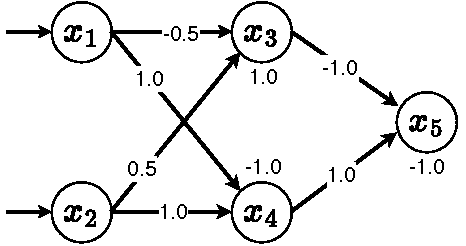
\includegraphics[width=0.5\linewidth]{figure/dnn.pdf}
    \caption{\label{fig:dnn} An FNN with ReLU.}
\end{figure}


\section{Types of Neural Networks}


\paragraph{Feed-Forward Network (FFN)} In an FFN information flows in one direction, from the input layer to hidden layers to the output layer (and thus no cycle).  

A fully connected feed-forward neural network (FNN), shown below, is an FFN where every neuron in a layer is connected to every neuron in the next layer.
\begin{center}
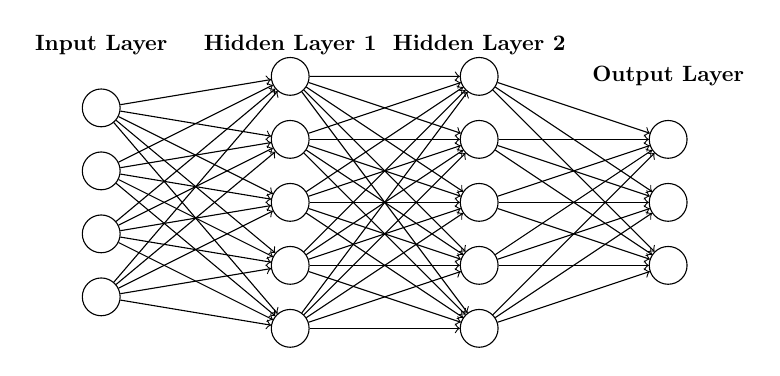
\begin{tikzpicture}[scale=0.8, transform shape]
% Input Layer
\node at (0,4) {\textbf{Input Layer}};
\foreach \x in {1,2,3,4} {
    \node[circle, draw=black, fill=white, minimum size=0.6cm] (I\x) at (0,4-\x) {};
}

% Hidden Layer 1
\node at (3,4) {\textbf{Hidden Layer 1}};
\foreach \x in {1,2,3,4,5} {
    \node[circle, draw=black, fill=white, minimum size=0.6cm] (H1\x) at (3,4.5-\x) {};
}

% Hidden Layer 2
\node at (6,4) {\textbf{Hidden Layer 2}};
\foreach \x in {1,2,3,4,5} {
    \node[circle, draw=black, fill=white, minimum size=0.6cm] (H2\x) at (6,4.5-\x) {};
}

% Output Layer
\node at (9,3.5) {\textbf{Output Layer}};
\foreach \x in {1,2,3} {
    \node[circle, draw=black, fill=white, minimum size=0.6cm] (O\x) at (9,3.5-\x) {};
}

% Connections
\foreach \i in {1,2,3,4}
    \foreach \j in {1,2,3,4,5}
        \draw[->] (I\i) -- (H1\j);

\foreach \i in {1,2,3,4,5}
    \foreach \j in {1,2,3,4,5}
        \draw[->] (H1\i) -- (H2\j);

\foreach \i in {1,2,3,4,5}
    \foreach \j in {1,2,3}
        \draw[->] (H2\i) -- (O\j);

\end{tikzpicture}
\end{center}





\paragraph{Convolutional Neural Networks (CNNs)} CNNs, often used in image recognition and classification, consist of neurons that have learnable weights and biases. Each neuron receives several inputs, takes a weighted sum over them, passes it through an activation function, and responds with an output.

\paragraph{Recurrent Neural Networks (RNNs)} RNNs, often used in natural language process and speech recognition, are designed to recognize patterns in sequences of data. RNNs have \emph{loops} in them, allowing information to be sent forward and backward.

\paragraph{Residual Networks} Residual Networks (ResNets) are a type of neural network that is often used in image recognition and classification. ResNets introduce skip connections that allow the gradient to flow directly through the network, making it easier to train deep networks.

\section{Properties of Neural Networks}
Similar to software programs, neural networks have desirable properties to ensure the network behaves as expected. These could be specific to the applications modeled by the network, e.g., safety properties in a collision avoidance system or general properties that are desired by all networks, e.g., robustness to adversarial attacks. 


\paragraph{Robustness Properties}
\emph{Robustness}, a desirable property for all networks, ensures that small perturbations in the input data do not cause major changes in the output of the network. For example, if a few pixels in an image are changed, the network should still classify the image correctly. \emph{Adversarial attacks} are a common way to test the robustness of a neural network. In an adversarial attack, an attacker makes small changes to the input data to cause the network to misclassify the data.

\emph{Local} robustness refers to robustness of a neural network within a \emph{small neighborhood or region} of the input data. In contrast, \emph{global} robustness refers to robustness of a network across the \emph{entire input space}. Global robustness is harder to achieve than local robustness, as it requires the network to be robust to all possible inputs.

\paragraph{$\epsilon$-robustness} A neural network is $\epsilon$-robust if the difference between any two inputs $x$ and $x'$ is within a small range $\epsilon$, the output $f$ of the network does not change significantly (or remain the same), i.e., $\|x-x'\| \leq \epsilon \implies f(x) \approx f(x')$.




\paragraph{Safety Properties} Safety properties are specific to the application modeled by the network. For example, a safety property in a collision avoidance system might be that if the intruder is distant and significantly slower than us, then we stay below a certain threshold, i.e., $d_{intruder} > d_{threshold} \land v_{intruder} < v_{threshold} \implies v_{us} < v_{threshold}$.


\subsection{Challenges}

\paragraph{Formalization}


\paragraph{Expressiveness}




\chapter{Verification of Neural Networks}\label{sec:verification}


\section{The Neural Network Verification (NNV) Problem}\label{sec:nnv-problem}
\paragraph{DNN Verification} Given a DNN \(N\) and a property $\phi$, the \emph{DNN verification problem} asks if $\phi$ is a valid property of $N$.
Typically, $\phi$ is a formula of the form $\phi_{in} \Rightarrow \phi_{out}$, where $\phi_{in}$ is a property over the inputs of $N$ and $\phi_{out}$ is a property over the outputs of $N$.
%This form of properties has been used to encode safety and security requirements of DNNs, e.g., safety specifications to avoid collision in unmanned aircraft~\cite{kochenderfer2012next} and \emph{adversarial robustness}~\cite{katz2017towards} properties desired by all DNNs, in which a small input perturbation does not cause major spikes in the DNN's outputs.
A DNN verifier attempts to find a \emph{counterexample} input to $N$ that satisfies $\phi_{in}$ but violates $\phi_{out}$.  If no such counterexample exists, $\phi$ is a valid property of $N$. Otherwise, $\phi$ is not valid and the counterexample can be used to retrain or debug the DNN~\cite{huang2017safety}.




% Verification tool such as Marabou and nnenum are then applied to the network to prove that the network is safe or identifier counterexample representing small input differences causing large output changes.


% \footnote{This is encoded as the differences of the inputs being within a certain small range  ($\phi_{in}$) implies the differences of the outputs still fall within a certain range in $\phi_{out}$)}.



\paragraph{Example} A valid property for the DNN in \autoref{fig:dnn} is that the output is $x_5 \le 0$ for any inputs $x_1 \in [-1,1], x_2\in[-2,2]$. An invalid property is that $x_5 > 0$ for those similar inputs.
A counterexample showing this property violation is $\{x_1=-1, x_2=2\}$, from which the DNN evaluates to $x_5=-3.5$. 

%Such properties can capture \emph{safety requirements} (e.g., a rule in an  collision avoidance system in~\cite{kochenderfer2012next,katz2017reluplex} is ``if the intruder is distant and significantly slower than us, then we stay below a certain threshold'') or \emph{local robustness}~\cite{katz2017towards} conditions (a form of adversarial robustness stating that small perturbations of a given input all yield the same output).


\section{Satisfiability and Activation Pattern Search}\label{sec:satisfiability-and-activation-pattern-search}

 As with traditional software, DNN verification is often represented as a satisfiability problem.
We thus need to define a formula to represent the network. Typically this formula is a conjunction of constraints representing the affine transformation and activation function of each neuron in the network.
For a network with $L$ layers, $N$ neurons per layer, and ReLU activations this formula is:
\begin{align*}
\alpha = \bigwedge_{\begin{smallmatrix}i \in [1,L]\\ j \in [1,N]\end{smallmatrix}} v_{i,j} = \max \Big( \sum_{k \in [1,N]} (w_{i-1,j,k} \cdot v_{i-1,j}) + b_{i,j}, 0 \Big)
\end{align*}
With this definition DNN verification can be formulated as checking the satisfiability of:
\begin{equation}\label{eq:prob}
  \alpha \land \phi_{in} \land \neg \phi_{out}
\end{equation}
If \autoref{eq:prob} is unsatisfiable, $\phi$ is a valid property of $\mathcal{N}$. Otherwise, $\phi$ is not valid (and the counterexample of the original problem is any satisfying assignment that makes \autoref{eq:prob} true).


\section{Activation Pattern Search} For the widely-used ReLU activation problem, the DNN verification problem becomes a search for \emph{activation patterns}, i.e., boolean assignments representing activation status of neurons, that lead to satisfaction the formula in \autoref{eq:prob}. 

Modern DNN verification techniques~\cite{bunel2020branch,wang2021beta,ferrari2022complete,duong2024harnessing,duong2023dpllt,ovalbab,katz2019marabou,bak2021nnenum} all adopt this idea and search for satisfying activation patterns.


\section{Complexity}

\chapter{Common Search Algorithms}

\section{Symbolic Search and Constraint solving}
\section{Branch-and-Bound (BnB)}

\begin{algorithm}[t]

    
    \SetKwData{nextlayer}{layer$_{i+1}$}
    \SetKwData{status}{status}
    \SetKwData{minimum}{objval}
    
    \SetKwFunction{InputMILP}{AddInputConstrs}
    \SetKwFunction{GetUnstableNeurons}{GetUnstableNeurons}
    \SetKwFunction{PiecewiseLinearMILP}{AddConstrsPWL}
    \SetKwFunction{LinearMILP}{AddConstrsLinear}
    \SetKwFunction{Maximize}{Maximize}
    \SetKwFunction{Minimize}{Minimize}
    \SetKwFunction{Feasible}{CheckFeasibility}
    \SetKwFunction{Optimize}{Optimize}
    \SetKwFunction{isPiecewiseLinear}{isPiecewiseLinear}
    \SetKwFunction{CreateStabilizedMILP}{CreateStabilizedMILP}
    \SetKwFunction{GetLeafNodes}{GetLeafNodes}
    \SetKwFunction{AddConstrs}{AddConstrs}
    \SetKwFunction{RemoveConstrs}{RemoveConstrs}
    \SetKwFunction{AddObjective}{AddObjectives}
    \SetKwFunction{ShortenSplitConstrs}{ShortenSplitConstrs}
    \SetKwFunction{RemoveLeafNodes}{RemoveLeaves}
    \SetKwFunction{StoppingConditions}{StoppingConditions}
    \SetKwFunction{RepOK}{RepOK}
    \SetKwFunction{RaiseError}{RaiseError}

    \SetKwInOut{Input}{input}
    \SetKwInOut{Output}{output}
    \SetKw{Break}{break}
    \SetKw{Continue}{continue}
    \SetKwFunction{Backtrack}{Backtrack}
    \SetKwFunction{Select}{Select}
    \SetKwFunction{Decide}{Decide}
    \SetKwFunction{BCP}{BCP}
    \SetKwFunction{Deduce}{Deduce}
    \SetKwFunction{AnalyzeConflict}{AnalyzeConflict}
    \SetKwFunction{BooleanAbstraction}{BooleanAbstraction}
    \SetKwFunction{AddClause}{AddClause}
    \SetKwFunction{isTotal}{isTotal}
    \SetKwFunction{randomattack}{RandomAttack}
    \SetKwFunction{pgd}{PGDAttack}
    
    \SetKwFunction{DPLLT}{DPLLT}
    \SetKwFunction{isValid}{isValid}
    \SetKwFunction{isEmpty}{isEmpty}
    \SetKwFunction{LPSolver}{LPSolver}
    \SetKwFunction{Solve}{Solve}
    \SetKwFunction{FindLayerNodes}{FindLayerNodes}
    \SetKwFunction{TightenInputBounds}{TightenInputBounds}
    \SetKwFunction{Abstract}{Abstract}
    \SetKwFunction{Check}{Check}
    \SetKwFunction{Decide}{Decide}
    \SetKwFunction{Imply}{Imply}
    \SetKwFunction{Lower}{LowerBound}
    \SetKwFunction{Upper}{UpperBound}
    \SetKwFunction{GetInputBounds}{GetInputBounds}
    \SetKwFunction{GetInputs}{GetInputs}
    \SetKwFunction{GetNumInputs}{GetNumInputs}
    \SetKwFunction{CurrentConflictClause}{CurrentConflictClause}
    \SetKwFunction{StopCriterion}{StopCriterion}
    \SetKwFunction{LastAssignedLiteral}{LastLiteral}
    \SetKwFunction{LiteralToVariable}{LiteralToVariable}
    \SetKwFunction{Antecedent}{Antecedent}
    \SetKwFunction{BinRes}{BinRes}
    \SetKwFunction{BacktrackLevel}{BacktrackLevel}
    \SetKwFunction{AddClause}{AddClause}
    \SetKwFunction{ActivationStatus}{ActivationStatus}
    \SetKwFunction{Backjump}{Backjump}
    \SetKwFunction{EstimateBounds}{EstimateBounds}
    
    \SetKwData{problems}{ActPatterns}
    \SetKwData{implicationgraph}{igraph}
    \SetKwData{literal}{lit}
    \SetKwData{variable}{var}
    \SetKwData{antecedent}{ante}
    \SetKwData{conflict}{conflict}
    \SetKwData{none}{none}
    \SetKwData{layerid}{lid}
    \SetKwData{hiddenbounds}{hidden\_bounds}
    \SetKwData{inputs}{inputs}
    \SetKwData{inputbounds}{input\_bounds}
    \SetKwData{outputbounds}{output\_bounds}
    \SetKwData{infeasible}{INFEASIBLE}
    \SetKwData{unreachable}{UNREACHABLE}
    \SetKwData{maxinputs}{MAX\_NUM\_INPUT}
    \SetKwData{assignment}{$\sigma$}
    \SetKwData{dl}{dl}
    \SetKwData{lpmodel}{solver}
    \SetKwData{clauses}{clauses}
    \SetKwData{conflict}{conflict}
    \SetKwData{clause}{clause}
    \SetKwData{igraph}{igraph}
    \SetKwData{cex}{cex}
    \SetKwData{sat}{sat}
    \SetKwData{unsat}{unsat}
    
    \SetKwData{submodel}{sub\_model}
    
    \SetKwData{true}{true}
    \SetKwData{false}{false}
    \DontPrintSemicolon
    
    \SetKwFunction{Restart}{Restart}
    
    \SetKwData{counterexample}{cex}
    \SetKwData{conflictclause}{conflict\_clause}
    \SetKwData{isconflict}{is\_conflict}

    \footnotesize
    \DontPrintSemicolon
  
    \Input{DNN $\mathcal{N}$, property $\phi_{in} \Rightarrow \phi_{out}$}
    \Output{$\unsat$ if property is valid, otherwise ($\sat, \counterexample$)}
    \BlankLine


    $\problems \leftarrow \{ \emptyset \}$ \tcp{initialize verification problems} 
    % $\prooftree \gets \{ ~ \}$ \tcp{initialize proof tree}\label{line:prooftree}
    
    \While(\tcp*[h]{main loop}){$\problems$}{\label{line:dpllstart}
        % \tcp{$\sigma_i$ is the activation pattern of problem $i$-th}
        $\sigma_i \gets \Select(\problems)$ \tcp{process problem $i$-th}
        % \Parfor(\tcp*[h]{process in parallel}){$\sigma_i ~\In~ \problems$}{ \label{line:parfor}
            \If{\Deduce{$\mathcal{N}, \phi_{in}, \phi_{out}, \sigma_i$}}{\label{line:deduce}
                $(\counterexample, v_i) \leftarrow \Decide(\mathcal{N}, \phi_{in}, \phi_{out}, \sigma_i)$ \\ \label{line:decide}
                \If(\tcp*[h]{found a valid counter-example}){$\counterexample$}{
                    \Return{$(\sat, \counterexample)$} 
                }
                \tcp{create new activation patterns}
                $\problems \leftarrow \problems \cup \{ \sigma_i \land v_i ~;~ \sigma_i \land \overline{v_i} \}$ \;
            }
            %\Else(\tcp*[h]{detect a conflict}){
                % $\clauses \leftarrow \clauses \cup \AnalyzeConflict(\igraph_i)$ \\ \label{line:analyze_conflict}
            %    $\prooftree \leftarrow \prooftree \cup \{ \sigma_i \}$ \tcp{build proof tree} \label{line:record_proof}
            %}
        % }
        % \If(\tcp*[h]{no more problems}){$\isEmpty(\problems)$}{
        % }
        
    }\label{line:dpllend}
    \Return{\unsat}
    
    \caption{The \dd{} algorithm.}\label{fig:alg}
\end{algorithm}

Most modern DNN verifiers adopt the branch-and-bound (BaB) approach to search for activation patterns for DNN verification. A BaB search consists of two main components: (branch) splitting into the problem smaller subproblems 
by using \emph{neuron splitting}, which decides boolean values representing neuron activation status, 
and (bound) using abstraction and LP solving to approximate bounds on neuron values to determine 
the satisfiability of the partial activation pattern formed by the split.


\autoref{fig:alg} shows \dd{}, a reference BaB architecture~\cite{nakagawa2014consolidating} for modern DNN verifiers. \dd{} takes as input a ReLU-based DNN $\mathcal{N}$ and a formulae $\phi_{in}\Rightarrow \phi_{out}$ representing the property of interest.
\dd{} iterates between (i) branching (\autoref{line:decide}), which \emph{decides} (assigns) an activation status value for a neuron, and (ii) bounding (\autoref{line:deduce}), which \emph{deduces} or checks the feasibility of the current activation pattern. 
%To add proof generation capability, \dd{} is instrumented with a proof tree (\texttt{proof}) variable (\autoref{line:prooftree}) to record these branching decisions. The proof is represented as a binary tree structure, where each node represents a neuron and its left and right edges represent its activation decision (active or inactive). %The proof tree is then used to generate a proof in the \nnproofformat{} format (\autoref{sec:proof-format}).




\begin{figure}[t]
    \begin{minipage}[b]{\linewidth}
        \centering
        \begin{minipage}[t]{0.48\textwidth}
            \centering  
            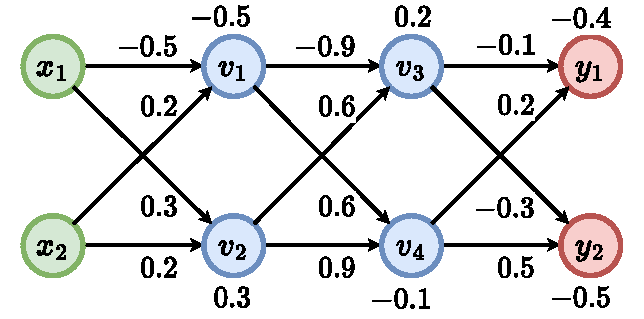
\includegraphics[width=\linewidth]{figure/proof_net.pdf}
            \caption*{(a)}
        \end{minipage}
        \begin{minipage}[t]{0.48\textwidth}
            \centering
            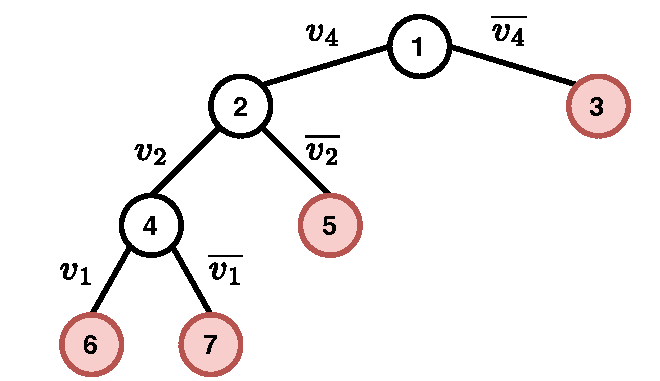
\includegraphics[width=\linewidth]{figure/proof_tree.pdf}
            \caption*{(b)}
        \end{minipage}
        \caption{(a) A simple DNN.  (b) A proof tree produced verifying the property $(x_1, x_2) \in [-2.0, 2.0] \times [-1.0, 1,0] \Rightarrow (y_1 > y_2)$.}
        \label{fig:example}
    \end{minipage}
\end{figure}
%White nodes correspond to branching nodes where \neuralsat{} makes decisions to split ReLU neurons.

\paragraph{Example} \autoref{fig:example}a illustrates a DNN and how \dd{} determines unsatisfiability (i.e., verifies the problem) and generates the unsat proof in \autoref{fig:example}b.

First, \dd{} initializes the activation pattern set \functiontextformat{ActPatterns} with an empty activation pattern $\emptyset$. Then \dd{} enters a loop (\autoref{line:dpllstart}-\autoref{line:dpllend}) to search for a satisfying assignment or a proof of unsatisfiability. In the first iteration, \dd{} selects the only available activation pattern $\emptyset \in \functiontextformat{ActPatterns}$. 
It calls \functiontextformat{Deduce} to check the feasibility of the problem based on the current activation pattern. \functiontextformat{Deduce} uses abstraction to approximate that from the input constraints the output values are feasible for the given network. 
Since \functiontextformat{Deduce} cannot decide infeasibility, \dd{} randomly selects a neuron to split (\functiontextformat{Decide}). Let us assume that it chooses $v_4$ to split, which essentially means the problem is split into two independent subproblems: one with $v_4$ active and the other with $v_4$ inactive.
\dd{} then adds $\{v_4\}$ and $\{\overline{v_4}\}$ to \functiontextformat{ActPatterns}.

In the second iteration, \dd{} has two subproblems (that can be processed in parallel). For the first subproblem with $v_4$, \functiontextformat{Deduce} cannot decide infeasibility, so it selects $v_2$ to split. It then conjoins $v_4$ with $v_2$ and then with $\overline{v_2}$ and adds both conjuncts to \texttt{ActPatterns}. 
For the second subproblem with $\overline{v_4}$ inactive, \functiontextformat{Deduce} determines that the problem is unsatisfiable and \dd{} saves the node $v_4$ to the proof tree, as node 3, to indicate one unsatisfiable pattern, i.e., whenever the network has $v_4$ being inactive, the problem is unsatisfiable.

In the third iteration, \dd{} has two subproblems for $v_4 \land v_2$ and $v_4 \land \overline{v_2}$. For the first subproblem, \functiontextformat{Deduce} cannot decide infeasibility, so it selects $v_1$ to split. It then conjoins $v_1$ and then $\overline{v_1}$ to the current activation pattern and adds them to \functiontextformat{ActPatterns}. For the second subproblem, \functiontextformat{Deduce} determines that the problem is unsatisfiable and \dd{} saves the node $v_4 \land \overline{v_2}$ to the proof tree, as node 5.

In the fourth iteration, \dd{} has two subproblems for $v_4 \land v_2 \land v_1$ and $v_4 \land v_2 \land \overline{v_1}$. Both subproblems are determined to be unsatisfiable, and \dd{} saves them to the proof tree as nodes 6 and 7, respectively.

Finally, \dd{} has an empty \texttt{ActPatterns}, stops the search, and returns \texttt{unsat} and the proof tree. 




\part{Optimizations and Strategies}


\chapter{GPU and Multicore Parallelism}


\part{Survey of DNN Verification Tools}

\chapter{Popular Techniques and Tools}
\chapter{Verifying the Verifiers}\label{sec:verifying-verifiers}





As discussed in previous chapters, advances in DNN verification have made it possible to reason about the safety and robustness of complex 
DNNs. However, as DNN tools become more complex (e.g., SOTA tools have 20K LoCs), they are more prone to bugs. The 2023 Neural Network Verification competition VNN-COMP'23~\cite{brix2023fourth} showed that 3 of the top 7 participants produced unsound results, incorrectly claiming unsafe DNNs are safe. This undesirable behavior defeats the purpose of DNN verification and hinders its practical adoption.

While all DNN verifiers can provide correct counterexamples for invalid properties, certifying valid results---proving no counterexample exists---is far more challenging, and no current verifiers can do this. This would require verifiers to track their decision steps, which are often complex and large. Moreover, each verification technique (e.g., branch and bound, conflict-driven learning, abstraction and refinement) would need a different proof generation approach, making it difficult to standardize and compare results across different tools.
This is unlike SAT solving, where most tools adopt the standard DPLL framework and thus allows for unified techniques in proof generation and checking (e.g., the DRAT family of algorithms for UNSAT proofs).







%\paragraph{Preliminary and Proposed Work}  We have developed \tool{}, a conflict-driven DNN verification tool that won the New Comer Award in VNN-COMP'23. Recently, we have added a proof generation technique, called \prooftool{}, to \tool{} to produce proofs for its validity  results. This proposal builds on these ideas to develop a comprehensive proof certification technique for DNN verifiers, making them trustworthy and reliable for safety-critical applications.

\part{Proof Generation and Checking}

\section{Proof Generation}\label{sec:proofgen}


Despite being well-tested, DNN verification tools are complex and may contain bugs. We propose a proof generation approach that can be used to generate a proof of the verification result. 
All of the major DNN verification approaches including: \crown{}~\cite{wang2021beta}, \neuralsat{}~\cite{duong2023dpllt}, \mnbab{}~\cite{ferrari2022complete}, \ovalnnv{}~\cite{ovalbab}, \nnenum{}~\cite{bak2021nnenum}, and \marabou{}~\cite{katz2019marabou}, share a common ``branch and bound'' (BaB) search structure: (i) (branch) split into smaller subproblems by using \emph{neuron splitting}, which decides boolean values representing neuron activation status, and (ii) (bound) use abstraction and LP solving to approximate bounds on neuron values to determine the satisfiability of the partial activation pattern formed by the split.
We leverage this commonality to bring proof generation capabilities with minimal overhead to existing DNN verification tools.

We focus on checking proofs of unsatisfiability (unsat) in this paper. 
A counterexample, $c$, returned by a verifier is an input that is purported to violate
the property.
This constitutes a proof of satisfiability (sat) 
which can easily be checked by evaluating $\phi(c,N(c))$.
In fact, VNN-COMP already requires competing DNN verification tools to return counterexamples demonstrating satisfiability.  In contrast, the proof of an unsatisfiability result (which explains why \emph{no possible inputs} can violate the property) is inherently more complex to generate (\autoref{sec:proof-gen}), requires a more sophisticated encoding (\autoref{sec:proof-format}), and an efficient checking algorithm (\autoref{sec:proof-checker}).

%\nnproofgen{} exploits 



%While multiple DNN verification approaches exist (e.g., simplex-based~\cite{katz2017reluplex,katz2022reluplex}, ~\cite{bunel2020branch,wang2021beta,ferrari2022complete}, and others ~\autoref{sec:related}), they all share a common structure: they use \emph{neuron splitting} (or \emph{case splitting}) to split the problem into smaller subproblems (like a search tree). %More specifically, they iteratively assign boolean values to neurons (true means active and false means inactive) and check the satisfiability of the DNN problem with the boolean assignment.
%For example, the ``branch'' in the popular class of  branch-and-bound (BaB)-based DNN verification techniques~\cite{bunel2020branch,wang2021beta,ferrari2022complete,duong2024harnessing,duong2023dpllt,ovalbab} refers to neuron splitting (while the ``bound'' refers to abstraction to approximate neural bounds).  
%\nnproofchecker{} is designed for neuron-splitting approaches and give these tools the ability to generate certified results with minimal overhead.






\SetKwInOut{Input}{input}
\SetKwInOut{Output}{output}
\SetKw{Break}{break}
\SetKw{Continue}{continue}
\SetKwFunction{Backtrack}{Backtrack}
\SetKwFunction{Select}{Select}
\SetKwFunction{Decide}{Decide}
\SetKwFunction{BCP}{BCP}
\SetKwFunction{Deduce}{Deduce}
\SetKwFunction{AnalyzeConflict}{AnalyzeConflict}
\SetKwFunction{BooleanAbstraction}{BooleanAbstraction}
\SetKwFunction{AddClause}{AddClause}
\SetKwFunction{isTotal}{isTotal}
\SetKwFunction{randomattack}{RandomAttack}
\SetKwFunction{pgd}{PGDAttack}

\SetKwFunction{DPLLT}{DPLLT}
\SetKwFunction{isValid}{isValid}
\SetKwFunction{isEmpty}{isEmpty}
\SetKwFunction{LPSolver}{LPSolver}
\SetKwFunction{Solve}{Solve}
\SetKwFunction{FindLayerNodes}{FindLayerNodes}
\SetKwFunction{TightenInputBounds}{TightenInputBounds}
\SetKwFunction{Abstract}{Abstract}
\SetKwFunction{Check}{Check}
\SetKwFunction{Decide}{Decide}
\SetKwFunction{Imply}{Imply}
\SetKwFunction{Lower}{LowerBound}
\SetKwFunction{Upper}{UpperBound}
\SetKwFunction{GetInputBounds}{GetInputBounds}
\SetKwFunction{GetInputs}{GetInputs}
\SetKwFunction{GetNumInputs}{GetNumInputs}
\SetKwFunction{CurrentConflictClause}{CurrentConflictClause}
\SetKwFunction{StopCriterion}{StopCriterion}
\SetKwFunction{LastAssignedLiteral}{LastLiteral}
\SetKwFunction{LiteralToVariable}{LiteralToVariable}
\SetKwFunction{Antecedent}{Antecedent}
\SetKwFunction{BinRes}{BinRes}
\SetKwFunction{BacktrackLevel}{BacktrackLevel}
\SetKwFunction{AddClause}{AddClause}
\SetKwFunction{ActivationStatus}{ActivationStatus}
\SetKwFunction{Backjump}{Backjump}
\SetKwFunction{EstimateBounds}{EstimateBounds}

\SetKwData{problems}{ActPatterns}
\SetKwData{implicationgraph}{igraph}
\SetKwData{literal}{lit}
\SetKwData{variable}{var}
\SetKwData{antecedent}{ante}
\SetKwData{conflict}{conflict}
\SetKwData{none}{none}
\SetKwData{layerid}{lid}
\SetKwData{hiddenbounds}{hidden\_bounds}
\SetKwData{layerbounds}{layer\_bounds}
\SetKwData{inputs}{inputs}
\SetKwData{inputbounds}{input\_bounds}
\SetKwData{outputbounds}{output\_bounds}
\SetKwData{infeasible}{INFEASIBLE}
\SetKwData{unreachable}{UNREACHABLE}
\SetKwData{maxinputs}{MAX\_NUM\_INPUT}
\SetKwData{assignment}{$\sigma$}
\SetKwData{dl}{dl}
\SetKwData{lpmodel}{solver}
\SetKwData{clauses}{clauses}
\SetKwData{conflict}{conflict}
\SetKwData{clause}{clause}
\SetKwData{igraph}{igraph}
\SetKwData{cex}{cex}
\SetKwData{sat}{sat}
\SetKwData{unsat}{unsat}
\SetKwData{certified}{certified}
\SetKwData{uncertified}{uncertified}
\SetKwData{submodel}{sub\_model}

\SetKwData{true}{true}
\SetKwData{false}{false}
\DontPrintSemicolon

\SetKwFunction{Restart}{Restart}

\SetKwData{counterexample}{cex}
\SetKwData{conflictclause}{conflict\_clause}
\SetKwData{isconflict}{is\_conflict}



\begin{algorithm}[t]
    \footnotesize
    \DontPrintSemicolon
  
    \Input{DNN $\mathcal{N}$, property $\phi_{in} \Rightarrow \phi_{out}$}
    \Output{($\unsat, \prooftree$) if property is valid, otherwise ($\sat, \counterexample$)}
    \BlankLine


    $\problems \leftarrow \{ \emptyset \}$ \tcp{initialize verification problems} 
    $\prooftree \gets \{ ~ \}$ \tcp{initialize proof tree}\label{line:prooftree}
    
    \While(\tcp*[h]{main loop}){$\problems$}{\label{line:dpllstart}
        % \tcp{$\sigma_i$ is the activation pattern of problem $i$-th}
        $\sigma_i \gets \Select(\problems)$ \tcp{process problem $i$-th}
        % \Parfor(\tcp*[h]{process in parallel}){$\sigma_i ~\In~ \problems$}{ \label{line:parfor}
            \If{\Deduce{$\mathcal{N}, \phi_{in}, \phi_{out}, \sigma_i$}}{\label{line:deduce}
                $(\counterexample, v_i) \leftarrow \Decide(\mathcal{N}, \phi_{in}, \phi_{out}, \sigma_i)$ \\ \label{line:decide}
                \If(\tcp*[h]{found a valid counter-example}){$\counterexample$}{
                    \Return{$(\sat, \counterexample)$} 
                }
                \tcp{create new activation patterns}
                $\problems \leftarrow \problems \cup \{ \sigma_i \land v_i ~;~ \sigma_i \land \overline{v_i} \}$ \;
            }
            \Else(\tcp*[h]{detect a conflict}){
                % $\clauses \leftarrow \clauses \cup \AnalyzeConflict(\igraph_i)$ \\ \label{line:analyze_conflict}
                $\prooftree \leftarrow \prooftree \cup \{ \sigma_i \}$ \tcp{build proof tree} \label{line:record_proof}
            }
        % }
        % \If(\tcp*[h]{no more problems}){$\isEmpty(\problems)$}{
        % }
        
    }\label{line:dpllend}
    \Return{$(\unsat, \prooftree)$}
    
    \caption{The \dd{} algorithm with proof generation.}\label{fig:alg}
\end{algorithm}



%\emph{Branch-and-bound} (BaB) is a common approach to DNN verification and used by major DNN verification tools including~\cite{bunel2020branch,wang2021beta,ferrari2022complete,duong2024harnessing,duong2023dpllt,ovalbab}.
%In BaB algorithms, ``branch'' means splitting the problem into smaller subproblems (like a search tree), and ``bound'' means computing the upper and lower bounds, using abstraction, of the problem to prune the search space. 



%Among modern DNN verification techniques, only the simplex-based approach attempts to generate proofs~\cite{desmartin2023towards,barbosa2023generating}. However, generating a proof for simplex-based approaches is non-trivial and incurs a significant overhead during the verification process~\cite{desmartin2023towards,barbosa2023generating}.

%Recently, an approach based on the DPLL(T) algorithm in SAT/SMT solving has shown much promise~\cite{duong2023dpllt}. For example, in its debut year, the DPLL(T)-based \neuralsat{} DNN verifier~\cite{duong2023dpllt} won the New Comer Award at VNN-COMP'23~\cite{brix2023fourth} and outperformed other state-of-the-art DNN verification tools, especially for very large networks~\cite{duong2024harnessing}. More importantly, DPLL(T) approach maintains \emph{implication graph}, an internal data structure to keep track of assignments, which essentially represent a  proof of the verification result. In other words, proofs are a built-in feature of DPLL(T) approach, and thus can be generated with minimal (in fact, \emph{zero}) overhead.

\subsection{Neuron-Splitting DNN Verification}\label{sec:bab}
\autoref{fig:alg} shows \dd{}, a reference architecture~\cite{nakagawa2014consolidating} 
for modern DNN verifiers that we use to illustrate our observations.  
\dd{} takes as input a ReLU-based DNN $\mathcal{N}$ and a formulae $\phi_{in}\Rightarrow \phi_{out}$ representing the property of interest.

\dd{} iterates between two components: \texttt{Decide} (branching, \autoref{line:decide}), which decides (assigns) an activation status value for a neuron, and \texttt{Deduce} (bounding, \autoref{line:deduce}), which checks the feasibility of the current activation pattern. 
To add proof generation capability, \dd{} is instrumented with a proof tree (\texttt{proof}) variable (\autoref{line:prooftree}) to record these branching decisions. The proof is represented as a binary tree structure, where each node represents a neuron and its left and right edges represent its activation decision (active or inactive). %The proof tree is then used to generate a proof in the \nnproofformat{} format (\autoref{sec:proof-format}).




\begin{figure}[t]
    \begin{minipage}[b]{\linewidth}
        \centering
        \begin{minipage}[t]{0.48\textwidth}
            \centering  
            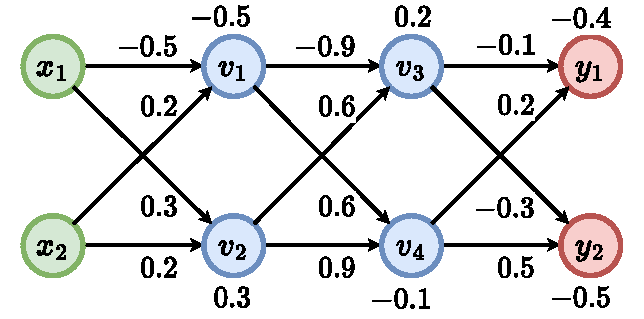
\includegraphics[width=\linewidth]{figure/proof_net.pdf}
            \caption*{(a)}
        \end{minipage}
        \begin{minipage}[t]{0.48\textwidth}
            \centering
            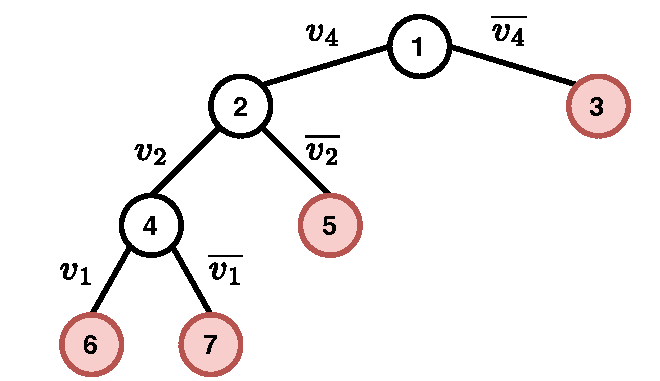
\includegraphics[width=\linewidth]{figure/proof_tree.pdf}
            \caption*{(b)}
        \end{minipage}
        \caption{(a) A simple DNN.  (b) A proof tree produced verifying the property $(x_1, x_2) \in [-2.0, 2.0] \times [-1.0, 1,0] \Rightarrow (y_1 > y_2)$.}
        \label{fig:example}
    \end{minipage}
\end{figure}
%White nodes correspond to branching nodes where \neuralsat{} makes decisions to split ReLU neurons.

\paragraph{Example} \autoref{fig:example}a illustrates a DNN and how \dd{} determines unsatisfiability (i.e., verifies the problem) and generates the unsat proof in \autoref{fig:example}b.

First, \dd{} initializes the activation pattern set \functiontextformat{ActPatterns} with an empty activation pattern $\emptyset$. Then \dd{} enters a loop (\autoref{line:dpllstart}-\autoref{line:dpllend}) to search for a satisfying assignment or a proof of unsatisfiability. In the first iteration, \dd{} selects the only available activation pattern $\emptyset \in \functiontextformat{ActPatterns}$. 
It calls \functiontextformat{Deduce} to check the feasibility of the problem based on the current activation pattern. \functiontextformat{Deduce} uses abstraction to approximate that from the input constraints the output values are feasible for the given network. 
Since \functiontextformat{Deduce} cannot decide infeasibility, \dd{} randomly selects a neuron to split (\functiontextformat{Decide}). Let us assume that it chooses $v_4$ to split, which essentially means the problem is split into two independent subproblems: one with $v_4$ active and the other with $v_4$ inactive.
\dd{} then adds $v_4$ and $\overline{v_4}$ to \functiontextformat{ActPatterns}.

In the second iteration, \dd{} has two subproblems (that can be processed in parallel). For the first subproblem with $v_4$, \functiontextformat{Deduce} cannot decide infeasibility, so it selects $v_2$ to split. It then conjoins $v_4$ with $v_2$ and then with $\overline{v_2}$ and adds both conjuncts to \texttt{ActPatterns}. 
For the second subproblem with $\overline{v_4}$ inactive, \functiontextformat{Deduce} determines that the problem is unsatisfiable and \dd{} saves the node $v_4$ to the proof tree, as node 3, to indicate one unsatisfiable pattern, i.e., whenever the network has $v_4$ being inactive, the problem is unsatisfiable.

In the third iteration, \dd{} has two subproblems for $v_4 \land v_2$ and $v_4 \land \overline{v_2}$. For the first subproblem, \functiontextformat{Deduce} cannot decide infeasibility, so it selects $v_1$ to split. It then conjoins $v_1$ and then $\overline{v_1}$ to the current activation pattern and adds them to \functiontextformat{ActPatterns}. For the second subproblem, \functiontextformat{Deduce} determines that the problem is unsatisfiable and \dd{} saves the node $v_4 \land \overline{v_2}$ to the proof tree, as node 5.

In the fourth iteration, \dd{} has two subproblems for $v_4 \land v_2 \land v_1$ and $v_4 \land v_2 \land \overline{v_1}$. Both subproblems are determined to be unsatisfiable, and \dd{} saves them to the proof tree as nodes 6 and 7, respectively.

Finally, \dd{} has an empty \texttt{ActPatterns}, stops the search, and returns \texttt{unsat} and the proof tree. 





\section{Proof Language}\label{sec:prooflang}

\lstdefinelanguage{SMTLIB}{
    morekeywords={assert, declare-const, declare-pwl, or, and, },
    alsoletter={-},
    morecomment=[l];,
    morestring=[b]",
    morekeywords=[2]{Real, Int, ReLU},
    keywordstyle=[2]\color{codepurple},
}

\lstdefinestyle{SMTLIB-style}{
    backgroundcolor=\color{backcolour},   
    commentstyle=\color{codegreen},
    keywordstyle=\color{blue},
    numberstyle=\tiny\color{black},
    stringstyle=\color{codepurple},
    basicstyle=\ttfamily\footnotesize,
    breakatwhitespace=false, 
    breaklines=true, 
    captionpos=b, 
    keepspaces=true, 
    numbers=left, 
    numbersep=5pt, 
    showspaces=false, 
    showstringspaces=false,
    showtabs=false, 
    tabsize=2,
}

\lstset{
    language=SMTLIB,
    style=SMTLIB-style
}

\newcommand{\lra}[1]{
    \textcolor{green!40!black}{\langle} 
    \textit{\textcolor{green!40!black}{#1}} 
    \textcolor{green!40!black}{\rangle}
}

\begin{figure}
{\small
\begin{align*}
    \lra{proof}         &::= \lra{declarations} \ \lra{assertions} \\
    \lra{declarations}  &::= \lra{declaration} \ | \ \lra{declaration} \ \lra{declarations} \\
    \lra{declaration}   &::= (\textbf{declare-const} \ \lra{input-vars} \ \textbf{Real}) \\
                        & \quad ~| \ (\textbf{declare-const} \ \lra{output-vars} \ \textbf{Real}) \\
                        & \quad ~| \ (\textbf{declare-pwl} \ \lra{hidden-vars} \ \lra{activation}) \\
    \lra{input-vars}    &::= \lra{input-var} \ | \ \lra{input-var} \ \lra{input-vars} \\
    \lra{output-vars}    &::= \lra{output-var} \ | \ \lra{output-var} \ \lra{output-vars} \\
    \lra{hidden-vars}    &::= \lra{hidden-var} \ | \ \lra{hidden-var} \ \lra{hidden-vars} \\
    \lra{activation}    &::= ~\text{ReLU} \ | \ \text{Leaky ReLU} \ | \ \ldots \\
    \lra{assertions}    &::= \lra{assertion} \ | \ \lra{assertion} \ \lra{assertions} \\
    \lra{assertion}     &::= (\textbf{assert} \ \lra{formula}) \\
    \lra{formula}       &::= (\lra{operator} \ \lra{term} \ \lra{term}) \\
                        & \quad ~| \ (\textbf{and} \ \lra{formula}+) \ | \ (\textbf{or} \ \lra{formula}+) \\
                        % & \quad ~| \ (\textbf{and} \ \lra{formula} \ \lra{formula}) \\
                        % & \quad ~| \ (\textbf{or} \ \lra{formula}+) \\
                        % & \quad ~| \ (\textbf{or} \ \lra{formula} \ \lra{formula}) \\
    \lra{term}          &::= \lra{input-var} \ | \ \lra{output-var} \\ 
                        & \quad ~| \ \lra{hidden-var} \ | \ \lra{constant} \\
    \lra{operator}      &::= ~ < \ | \ \leq \ | \ > \ | \ \geq \\
    \lra{input-var}     &::= ~\text{X\_}\lra{constant} \\
    \lra{output-var}    &::= ~\text{Y\_}\lra{constant} \\
    \lra{hidden-var}    &::= ~\text{N\_}\lra{constant} \\
    \lra{constant}      &::= ~\textbf{Int} \ | \ \textbf{Real}
\end{align*}
}
\caption{The \nnproofformat{} proof language.}\label{fig:grammar}
\end{figure}

We have shown that the broad class of DNN verification techniques represented by \dd{}
can generate a binary tree that represents a proof of unsatisfiability  (\autoref{sec:proof-structure}). 
Rather than record such proofs in an verifier-specific format, we define a standard format
that is human-readable, is compact, can be efficiently generated by verification tools, and can
be efficiently processed by proof checkers.  
To meet this goal, we introduce \nnproofformat{}, a proof language to specify DNN proofs.
This language is inspired by the SMTLIB format~\cite{barrett2010smt} used for SMT solving, which has also been adopted by the  VNNLIB language~\cite{vnnlib} to specify DNNs and their properties for  verification.

%accepted by our proof check algorithm (\autoref{sec:proof-checker}

\autoref{fig:grammar} outlines the \nnproofformat{} syntax and grammar, represented as production rules. 
A proof is composed of \textit{declarations} and \textit{assertions}. Declarations define the variables and their types within the proof. Specifically, \textit{input variables} (prefixed with \functiontextformat{X}) and \textit{output variables} (prefixed with \functiontextformat{Y}) are declared as real numbers, representing the inputs and outputs of the neural network, respectively. Additionally, \textit{hidden variables} are declared with specific piece-wise linear (PWL) activation functions, such as ReLU or Leaky ReLU. These hidden variables correspond to the internal nodes of the neural network that process the input data through various activation functions.

Assertions are logical statements that specify the conditions or properties that must hold within the proof. Assertions over input variables are \emph{preconditions} and those over output variables are \emph{post-conditions}. Each assertion is composed of a \textit{formula}, which can involve terms and logical operators. Formulas include simple comparisons between terms (e.g., less than, greater than) or more complex logical combinations using \functiontextformat{and} and \functiontextformat{or} operators. The terms used in these formulas can be input variables, output variables, hidden variables, or constants.

\begin{figure}
\begin{lstlisting}[style=SMTLIB-style, language=SMTLIB]
; Declare variables
(declare-const X_0 X_1 Real)
(declare-const Y_0 Y_1 Real)
(declare-pwl N_1 N_2 N_3 N_4 ReLU)

; Input constraints
(assert (>= X_0 -2.0))
(assert (<= X_0  2.0))
(assert (>= X_1 -1.0))
(assert (<= X_1  1.0))

; Output constraints
(assert (<= Y_0 Y_1)) 

; Hidden constraints
(assert (or 
    (and (<  N_4 0))
    (and (<  N_2 0) (>= N_4 0))
    (and (>= N_2 0) (>= N_1 0) (>= N_4 0))
    (and (>= N_2 0) (<  N_1 0) (>= N_4 0))))
\end{lstlisting}
\caption{\nnproofformat{} example format of the proof tree in \autoref{fig:example}b. 
%\tvn{seems to take too much space. Could we put multiple statements in a line?}\hd{is it compact enough?}\tvn{yep. thanks}
}
\label{fig:proof_example}
\end{figure}

%\autoref{fig:proof_example} shows an example of a proof in \nnproofformat{} using the network in \autoref{fig:example}a. 

The \texttt{declare-*} statements declare input, output, and hidden variables, while the \texttt{assert} statements specify the constraints on these variables (i.e., the pre and postcondition of the desired property).
The hidden constraints represent the activation patterns of the hidden neurons in the network (i.e., the proof tree). Each \texttt{and} statement represents a tree path that represents an activation pattern. 



\emph{Example}: The proof in \autoref{fig:proof_example} corresponds to the proof tree in \autoref{fig:example}b. The statement \texttt{(and (< N\_4 0))} corresponds to the rightmost path of the tree with $\overline{v_4}$ decision (leaf 3).  The statement \texttt{(and (< N\_2 0) (>= N\_4 0))} corresponds to the path with $v_4 \land \overline{v_2}$ (leaf 5). 

The \nnproofformat{} language is intentionally designed to (a) not explicitly include weights/bias terms to minimize size of the proof structure, and (b) explicitly reflect a DNF structure to enable easy parallelization.
The DNN weight and bias terms are readily available in the ONNX~\cite{onnx} format, which can be accessed by any \nnproofformat{} checker like the one we describe next.


\section{Proof Checker}\label{sec:proofchecker}
Finally, we need to check that the generated proof is correct and that the original DNN verification problem is indeed unsatisfiable. The checker must be efficient to handle large proofs and trusted of its results (if it verifies the proof, then the original DNNV problem is proved).
To achieve this, we will develop a proof checker call \proofcheck{} to validate \prooflang{} proofs.
\proofcheck{} will be verifier-independent and support \prooflang{} proofs generated by different verification tools. 



We introduce a proof checker, \nnproofchecker{}, that validates \nnproofformat{} proofs generated by DNN verification tools.
\nnproofchecker{} is verifier-independent and can check \nnproofformat{} proofs generated by a wide-range of verification tools.
It is also efficient and scales to handle large proof trees.

\subsection{The Core \nnproofcheck{} Algorithm}


The goal of \nnproofcheck{} is to verify that the \nnproofformat{} tree generated by a DNN verification tool is correct (i.e., the proof tree is a proof of unsatisfiability of the DNN verification problem).
\nnproofcheck{} thus must verify that the constraint represented by each \emph{leaf} node in the proof tree is unsatisfiable. To check each node, \nnproofcheck{} forms an MILP problem (\autoref{sec:milp}) consisting of the constraint in \autoref{eq:prob} (the DNN, the input condition, and the negation of the output) with the constraints representing the activation pattern encoded by the tree path to the leaf node. \nnproofcheck{} then invokes an LP solver to check that the MILP problem is infeasible, which indicates unsatisfiability of the leaf node. 

\begin{algorithm}[t]
    \footnotesize

    \Input{DNN $\mathcal{N}$, property $\phi_{in} \Rightarrow \phi_{out}$, $\prooftree$}
    \Output{\certified if proof is valid, otherwise \uncertified}
    \BlankLine

    \If{$\neg$ \RepOK(\prooftree)}{
        \RaiseError{Invalid proof tree}
    }

    \tcp{initialize MILP model with inputs}
    $\model \leftarrow \CreateStabilizedMILP(\mathcal{N}, \phi_{in}, \phi_{out})$ \label{line:build_model}

    
    $\leaf \gets \mynull$ \tcp{initialize current processing node}
    
    \While{$\prooftree$}{\label{line:proof_loop}
        
        % \tcp{Get $k$ leaf nodes from $\prooftree$}
        % $[\leaf_1, ..., \leaf_k] \gets \GetLeafNodes(\prooftree, k)$ \\ \label{line:get_leaf}
        $\leaf \gets \Select(\prooftree, \leaf)$ \tcp{get next node to check} \label{line:select} \label{line:get_leaf}

        % \tcp{Process $k$ nodes in parallel}
        % \Parfor{$\leaf_i ~\In~ [\leaf_1, ..., \leaf_k]$}{ \label{line:parfor}
        
        $\model \gets \AddConstrs(\model, \leaf)$  \tcp{add constraints} \label{line:add_proof_leaf_constrs}
        
        % $\minimum \gets \Minimize(\model)$ \tcp{} \label{line:optimize1}
        \If{$\Feasible(\model)$}{\label{line:proof_check_objective1}
            \Return{\uncertified} \tcp{cannot certify}
        }
        
        % $\Backtrack(\prooftree, \leaf)$ \tcp{process interior node}
        
        % \While{$\StoppingConditions(\leaf_i)$}{ \label{line:stop_condition}
        %     % \tcp{remove constraints of old $\leaf_i$ }
        %     % $\model \gets \RemoveConstrs(\model, \leaf_i)$  \\
        %     % \tcp{move to $\leaf_i$'s parent}
        %     % $\leaf_i \gets \ShortenSplitConstrs(\leaf_i)$ \\
        %     % \tcp{add constraints of new (looser) $\leaf_i$ }

        %     \tcp{move to $\leaf_i$'s parent}
        %     $\model \gets \Backjump(\leaf_i)$  \\ \label{line:proof_backjump}

        %     \tcp{Prove the new $\leaf_i$}
        %     $\minimum \gets \Minimize(\model)$ \\ \label{line:optimize2}
        %     \If(\tcp*[h]{cannot certify}){$\minimum \le 0$}{
        %         \Break
        %     }
        %     \tcp{if parent is proved, remove its children}
        %     $\prooftree \gets \RemoveLeafNodes(\prooftree, \leaf_i)$ \label{line:proof_prune}
        % }
        }
    % }
    \Return{\certified}

    \caption{\nnproofcheck{} algorithm.}
    % \Description{}
    \label{fig:algorithm}
\end{algorithm}


\autoref{fig:algorithm} shows a minimal (core)  \nnproofcheck{} algorithm, which takes as input a DNN $\mathcal{N}$, a property $\phi_{in} \Rightarrow \phi_{out}$, a proof tree $\prooftree$, and returns \certified if the proof tree is valid and \uncertified otherwise. 
\nnproofcheck{} first checks the validity of the proof tree (\autoref{line:build_model}), i.e., the input must represent a proper \nnproofformat{} proof tree (\autoref{sec:proof-format}).  
If the proof tree is invalid, \nnproofcheck{} raises an error.
\nnproofcheck{} next creates a MILP model (\autoref{line:build_model}) representing the input. % (\autoref{sec:neuron-stabelization}).
\nnproofcheck{} then enters a loop (\autoref{line:proof_loop}) that selects a (random) leaf node from the proof tree (\autoref{line:select}) and adds its MILP constraint to the model (\autoref{line:add_proof_leaf_constrs}). It then checks the model using an LP solver to determine whether the leaf node is unsatisfiable. If the LP solver returns feasibility, \nnproofcheck{} returns \uncertified, i.e., it cannot verify the input proof tree. 
\nnproofcheck{} continues until all leaf nodes are checked and returns \certified, indicating the proof tree is valid.



\subsubsection{Example} For the \nnproofformat{} proof in \autoref{fig:proof_example}, we need to check that the four leaf nodes 3, 5, 6, and 7 of the proof tree in \autoref{fig:example}b are unsatisfiability. Assume \nnproofcheck{} first selects node 3, it forms the MILP problem for leaf node 3 by conjoining the constraint representing $0.6v_1 + 0.9v_2 - 0.1 \le 0$ (i.e., $\overline{v_4}$) %\tvn{Hai check}\hd{by setting $a_1^{(2)}=0$ representing that $\hat{z}_1^{(2)} \le 0$ (see \autoref{eq:mip}e) or \emph{implicitly} conjoining the inequality $0.6\hat{z}^{(1)}_0 + 0.9\hat{z}^{(1)}_1 - 0.1 \le 0$ (or ${z}_1^{(2)} \le 0$), where $\hat{z}^{(1)}_0$, $\hat{z}^{(1)}_1$ represent the outputs of $v_1$ and $v_2$, respectively.} 
with the constraints in \autoref{eq:prob} representing the input ranges and the DNN with the objective of optimizing the output. \nnproofcheck{} then invokes an LP solver, which determines that this MILP is infeasible, i.e., leaf node 3 indeed leads to unsatisfiability. \nnproofcheck{} continues this process for the other three leaf nodes and returns \certified as all leaf nodes are unsatisfiable.


\subsubsection{MILP Formulation}\label{sec:milp}

\nnproofcheck{} formulates MILP problems~\cite{tjeng2019evaluating} and check for feasible solutions using off-the-shelf LP solving. Formally, the MILP problem is defined as:
\begin{equation}
    \begin{aligned}
        &\mbox{(a)}\quad z^{(i)} = W^{(i)} \hat{z}^{(i-i)} + b^{(i)};\\
        &\mbox{(b)}\quad y = z^{(L)};  x = \hat{z}^{(0)}; \\
        &\mbox{(c)}\quad \hat{z}_j^{(i)} \ge {z}_j^{(i)}; \hat{z}_j^{(i)} \ge 0; \\
        &\mbox{(d)}\quad a_j^{(i)} \in \{ 0, 1\} ;\\
        &\mbox{(e)}\quad \hat{z}_j^{(i)} \le {a}_j^{(i)} {u}_j^{(i)}; \hat{z}_j^{(i)} \le {z}_j^{(i)} - {l}_j^{(i)}(1 - {a}_j^{(i)}); \\
    \end{aligned}
    \label{eq:mip}
\end{equation}

\noindent where $x$ is input, $y$ is output, and $z^{(i)}$, $\hat{z}^{(i)}$, $W^{(i)}$, and $b^{(i)}$ are the pre-activation, post-activation, weight, and bias vectors for layer $i$, respectively. 
This encodes the semantics of a ReLU-based DNN:  
(a) the affine transformation computing the pre-activation value for a neuron in terms of outputs in the preceding layer;
(b) the inputs and outputs in terms of the adjacent hidden layers;
(c) assertion that post-activation values are non-negative and no less than pre-activation values;
(d) neuron activation status indicator variables that are either 0 or 1; and
(e) constraints on the upper, $u_j^{(i)}$, and lower, $l_j^{(i)}$, bounds of the pre-activation value of the $j$th neuron in the $i$th layer.
Deactivating a neuron, $a_j^{(i)} = 0$, simplifies the first of the (e) constraints to $\hat{z}_j^{(i)} \le 0$, and activating a neuron simplifies the second to $\hat{z}_j^{(i)} \le z_j^{(i)}$, which is consistent with the semantics of $\hat{z}_j^{(i)} = max(z_j^{(i)},0)$.


\subsubsection{Correctness}\label{sec:checker-core-correctness}

 \autoref{fig:algorithm} returns \certified iff the input \nnproofformat{} proof tree is unsatisfiable. This proof tree encodes a disjunction of constraints, one per tree path, where each constraint represents an activation pattern of the network (the leaf node). The algorithm checks each constraint using LP solving and only returns certified iff every one of them is unsatisfiable.  
%Moreover, while pruning optimization (\autoref{sec:pruning}) in \autoref{fig:algorithm} allows the checker to skip children nodes if the parent node is unsatisfiable, this is still sound because the structure of the proof tree guarantees that the constraints of a child is more restricted its parent, and thus if the parent node is unsatisfiable, the children nodes must also be unsatisfiable. The algorithm  terminates because the proof tree (or the DNF) is finite and the checker will eventually check all nodes.
We note that this correctness argument assumes that the LP solver is correct -- in practice
multiple solvers could be used to guard against errors in that component.  We note that
it is standard for proof checkers to assume the correctness of a small set of external tools, e.g., checkers that use  theorem provers assume the correctness of the underlying prover~\cite{lammich2023grat}.

\subsection{Optimizations}
While the core \nnproofcheck{} algorithm in \autoref{fig:algorithm} is minimal, it can be inefficient. \nnproofchecker{} employs several optimizations to improve its efficiency. These are crucial for checking large proof trees generated by DNN verification tools for challenging problems.


\subsubsection{Neuron Stabilization}\label{sec:neuron-stabelization} 

\begin{algorithm}[t]
    \footnotesize

    \Input{DNN $\mathcal{N}$, property $\phi_{in} \Rightarrow \phi_{out}$, parallel factor $k$}
    \Output{MILP $\model$}
    \BlankLine
    

    $\model \leftarrow \InputMILP(\phi_{in})$  \tcp{input property}    \label{line:create_input}

    \tcp{Add MILP constraints for each layer of network}
    \For{$\layer ~\In ~\mathcal{N}$}{
        \If{$\isPiecewiseLinear(\layer)$}{
            \tcp{add constraints \autoref{eq:mip} (c), (d), (e)} 
            $\model \leftarrow \PiecewiseLinearMILP(\layer, \phi_{in}, \phi_{out})$ \\ \label{line:create_pwl_layer}
        }
        \Else(\tcp*[h]{this layer is linear}){
            \tcp{add constraints \autoref{eq:mip} (a), (b)} 
            $\model \leftarrow \LinearMILP(\layer, \phi_{in}, \phi_{out})$ \\ \label{line:create_linear_layer}

            \tcp{estimate upper and lower bounds} 
            $\layerbounds \gets \EstimateBounds(\layer)$ \\ \label{line:estimate_bounds}
            
            \tcp{select unstable neurons to be stabilized} 
            $[v_1, ..., v_k] \leftarrow \GetUnstableNeurons(\layerbounds)$ \\ \label{line:find_unstable}
        
            \tcp{stabilize selected neurons in parallel}
            \Parfor{$v_i ~\In~[v_1, ..., v_k]$}{ \label{line:parallel_stabilize}
                % \tcp{lower is closer to 0 than upper}
                \tcp{optimize lower first}
                \If{$(v_i.lower + v_i.upper) \ge 0$}{
                    $\Maximize(\model, v_i.lower)$ \\ \label{line:maximize1}
                    \If(\tcp*[h]{still unstable}){$v_i.lower < 0$}{
                        $\Minimize(\model, v_i.upper)$ \label{line:minimize1}
                    }
                }
                % \tcp{upper is closer to 0 than lower}
                % \tcp{optimize upper first}
                \Else(\tcp*[h]{optimize upper first}){
                    $\Minimize(\model, v_i.upper)$ \\ \label{line:minimize2}
                    \If(\tcp*[h]{still unstable}){$v_i.upper > 0$}{
                        $\Maximize(\model, v_i.lower)$  \label{line:maximize2}
                    }
                }
            }
        }
    }

    $\model \gets \AddObjective(\model, \phi_{out})$ \tcp{output property}
    
    \Return{$\model$}
    
    % \vspace*{-0.2in}
    \caption{\texttt{CreateStabilizedMILP} procedure.}
    \label{fig:stabilize}
    % \Description{}
\end{algorithm}

A primary challenge in DNN analysis is the presence of large numbers of piecewise-linear constraints (e.g., ReLU) which generate a large number of branches and yield large proof trees. In the MILP formulation, this creates many disjunctions which are hard to solve. To reduce the number of disjunctions, \nnproofchecker{} uses \emph{neuron stabilization}~\cite{duong2024harnessing}
to determine neurons that are \emph{stable}, either active or inactive, for all inputs defined by the property pre-condition.
For all stable neurons, the disjunctive ReLU constraint is replaced with a linear constraint that represents the neuron's value.   This simplifies the MILP problem.

\nnproofchecker{} uses the algorithm in \autoref{fig:stabilize} to traverse the DNN and compute stable neurons. The algorithm initializes the MILP model with input constraints (\autoref{line:create_input}) and then iterates over each layer of the network. 
%follows the~\autoref{eq:mip} to create corresponding 
Next, for each layer, it creates constraints (\autoref{line:create_pwl_layer} or \autoref{line:create_linear_layer}) depending on the layer type.
Moreover,  it uses approximation to estimate bounds of neuron values to determine neuron stability (\autoref{line:estimate_bounds}).
Next, it filters unstable neurons (\autoref{line:find_unstable}) and attempt to make them stable by optimizing either their lower ($\Maximize$) or upper ($\Minimize$) bounds.



\subsubsection{Pruning Leaf Nodes}\label{sec:pruning}
%\hd{``Pruning'' sounds better}

Another optimization \nnproofchecker{} employs is that it does not check child nodes if the parent node is unsatisfiable.
In an \nnproofformat{} proof tree, a child node adds constraints to the parent (e.g., node 6 adds the constraint of $v_1$ to node 4, which adds the constraint of $v_2$ to node 2 in \autoref{fig:example}b). Thus, if we determine that the constraint of the parent is unsatisfiable, we can skip the child nodes, which must also be unsatisfiable.  

%Simply checking parent nodes would actually increase MILP cost, because they have shorter tree paths and thus have a greater number of disjunctive constraints.

\nnproofchecker{} uses a backtracking mechanism to check the parent node only when the child nodes are infeasible. Specifically, it starts checking a leaf node $l$. If it determines unsatisfiability it will check the parent $p$ of $l$. If $p$ is unsatisfiable it immediately removes the children of $p$ (more specifically the sibling of $l$). Next it backtracks to the parent of $p$ and repeats until meeting a stopping criteria. This optimization reduces the number of LP problems that need to be solved, making the proof checking process more efficient. 

We implement a backjumping strategy that allows for backtracking multiple levels, $N$, rather than a single level at a time.
A large value of $N$ offers the chance for greater pruning if an unsatisfiable node is found by
backjumping, but such nodes also represent less constrained, and therefore, more complex MILP problems
and are less likely to be unsatisfiable.
The default value in $\nnproofchecker{}$ is $N=2$ is selected to enable a modest degree of pruning,
while being close enough to a proven unsatisfiable node that it has a reasonable chance of itself being unsatisfiable.
Future work will explore tuning $N$ to a given verification problem.


% \hd{Without X, \nnproofchecker{} will have to check all the children.}

% \hd{It backjumps when the leave node is proved and X optimization is enabled. 
% We can keep backing up until it cannot prove anymore, however, after N times, each time half the length of an activation pattern, an activation pattern is shortened to $1 / 2^{N}$ (e.g., if $N=2$, after 2 times of backing up, an activation pattern is shortened to 1/4 of its length). 
% This is when the pruned leaves by those proved interiors are getting overlapped (due to parallelization, we backjump on multiple leaves), so more backjumps might not helpful. 
% Instead, we start over with a new iteration with remaining leaves.
% I experienced with $N = \{1, 2, 3, 4, 5\}$ and I settled down $N=2$ for all experiments (fixed N) which seems to be good enough in our experiments. 
% Increasing $N$ does not improve the performances but hurts especially when dealing with CNNs.
% }
% \matt{I think my main point is ``How much of this is important to \nnproofchecker{}?'' whatever is important needs to be described.  You don't need to describe all of the discarded alternatives.  If we settled on a particular strategy, then define that strategy and say why it works well, e.g., balances cost of failing to prove unsat for parents with ability to prune sub-trees.  Right now we just say "simple backtracking mechanism", but your description makes seem like it is not all that simple.}
% This optimization reduces the number of LP problems that need to be solved, making the proof checking process more efficient.

%. \nnproofchecker{} thus uses a simple backtracking mechanism to check the parent node only when the child nodes are infeasible. This optimization reduces the number of LP problems that need to be solved, making the proof checking process more efficient.
%However, checking the parent node is more expensive than checking the child nodes (otherwise we can just directly check the root node). \nnproofchecker{} thus uses a simple backtracking mechanism to check the parent node only when the child nodes are infeasible. This optimization reduces the number of LP problems that need to be solved, making the proof checking process more efficient.

\subsubsection{Parallelization} Finally, the structure of \nnproofformat{} proof tree is designed to be easily parallelized.  Each tree path is an independent sub-proof and partitions of the tree allow checker to leverage multiprocessing to check large proof trees efficiently. \nnproofchecker{} uses a parameter $k$ to control the number of leaf nodes to be checked in parallel.


\subsubsection{Correctness} These three optimizations preserve the correctness of the \nnproofcheck{} algorithm (\autoref{sec:checker-core-correctness}). First, neuron stabilization just simplifies the MILP problem and removes irrelevant, i.e., stable, neurons, which by definition are not affected by activation patterns. Second, while backtracking allows the checker to skip some nodes, this is sound because the structure of the proof tree guarantees that the constraints of a child is more restrictive than its parent, and thus if the parent is unsatisfiable, the children must also be. Finally, parallelization is sound because each tree path is independent and the checker will eventually check all nodes.

%\subsection{The \nnproofchecker{} Algorithm and Implementation}


\section{Evaluation}\label{sec:evaluation}  
Our goals are to understand how checking of \nnproofformat{}s performs, how it can be optimized, and how robust checking is to
verification optimizations.
We focus our evaluation on the following research questions:

\noindent\mbox{~~}\textbf{RQ1} (\autoref{sec:rq1}): How does \nnproofchecker{} perform and how does it compare prior work? 

\noindent\mbox{~~}\textbf{RQ2} (\autoref{sec:rq2}): How does proof checking optimization improve performance?

\noindent\mbox{~~}\textbf{RQ3} (\autoref{sec:rq3}): How does proof checking performance vary with verification algorithms and optimizations?



\subsection{Experimental Design}\label{sec:exp_design}
We describe the selection of benchmarks, baselines, metrics, and treatments used
to explore the above RQs.

\ignore{
\begin{table*}[t]
    \footnotesize
    \centering
    \caption{Benchmark instances. U: \texttt{unsat}, S: \texttt{sat}, ?: \texttt{unknown}.}\label{tab:benchmarks}
    % \vspace*{-3mm}
    % \resizebox{\textwidth}{!}{
    \begin{tabular}{c|ccrr|cc}
        \toprule
        % \multirow{2}{*}{\textbf{Benchmarks}} &\multicolumn{3}{c}{\textbf{Networks}}  &\multicolumn{2}{|c}{\textbf{Tasks}}\\
        % \multirow{2}{*}{\textbf{Benchmarks}} &\multicolumn{2}{c}{\textbf{Networks}} &  \multicolumn{2}{c|}{\textbf{Per Network}} &\multicolumn{2}{c}{\textbf{Tasks}}\\
        \multirow{2}{*}{\textbf{Benchmarks}} &\multicolumn{4}{c}{\textbf{Networks}} & \multicolumn{2}{|c}{\textbf{Tasks}}\\
        & Type & Networks & Neurons & Parameters & Properties & Instances (U/S/?)\\
  
        \midrule
        \multirow{4}{*}{FNN\_SMALL}         & \multirow{4}{*}{FNN + ReLU} & 2 x FNN(32) &   64 & 27K & 25 & 25/0/0 \\
                                            &                             & 4 x FNN(32) &  128 & 29K & 25 & 25/0/0 \\
                                            &                             & 2 x FNN(64) &  128 & 55K & 25 & 25/0/0 \\
                                            &                             & 4 x FNN(64) &  256 & 63K & 25 & 25/0/0 \\
        
        \midrule
        \multirow{4}{*}{FNN\_MEDIUM}        & \multirow{4}{*}{FNN + ReLU} & 2 x FNN(256)  &    512 &  269K & 25 & 25/0/0 \\
                                            &                             & 4 x FNN(256)  &   1024 &  401K & 25 & 25/0/0 \\
                                            &                             & 6 x FNN(256)  &   1536 &  532K & 25 & 25/0/0 \\
                                            &                             & 6 x FNN(512)  &   3072 & 1.7M & 25 & 25/0/0 \\
        \midrule
        \multirow{4}{*}{CNN\_SMALL}         & \multirow{4}{*}{CNN + ReLU} & 1 x CNN(3, 21), 1 x FNN(128)  &   320 & 27K & 25 & 25/0/0 \\
                                            &                             & 1 x CNN(3, 19), 1 x FNN(128)  &   428 & 41K & 25 & 25/0/0 \\
                                            &                             & 1 x CNN(3, 17), 1 x FNN(128)  &   560 & 58K & 25 & 25/0/0 \\
                                            &                             & 1 x CNN(3, 13), 1 x FNN(128)  &   896 & 100K & 25 & 25/0/0 \\
        \midrule
        \multirow{4}{*}{CNN\_MEDIUM}        & \multirow{4}{*}{CNN + ReLU} & 1 x CNN(3, 9), 1 x CNN(5, 11), 1 x FNN(128)  &   1828 & 67K & 25 & 25/0/0 \\
                                            &                             & 1 x CNN(3, 7), 1 x CNN(5, 9),  1 x FNN(128)  &   2560 & 128K & 25 & 25/0/0 \\
                                            &                             & 1 x CNN(5, 9), 1 x CNN(7, 11), 1 x FNN(128)  &   2828 & 96K & 25 & 25/0/0 \\
                                            &                             & 1 x CNN(5, 7), 1 x CNN(7, 9),  1 x FNN(128)  &   3920 & 180K & 25 & 25/0/0 \\
        \midrule
        \textbf{Total}                      &                             & \textbf{16}                  &     &   & \textbf{400} & \textbf{400/0/0} \\
        \bottomrule
    \end{tabular}
    % }
\end{table*}
}


\paragraph{Benchmarks}
Evaluating these research questions requires neural network verification problems
that are valid, i.e., their formulation as satisfiability problems is UNSAT.

The yearly VNN-COMP competitions~\cite{brix2023first,brix2023fourth,bak2021second} includes a wide-variety of benchmarks,
but the competitions organizers observed that many benchmarks are too easy.
They contain large numbers SAT problems that can be solved by adversarial attacks 
or UNSAT problems that can be solved, without any state splitting, using coarse overapproximations.
They conclude that there is a need 
for benchmarks to be ``not so easy that every tool can solve all of them''~\cite{brix2023first}.
For this reason, we base our benchmark selection on a recent paper~\cite{duong2024harnessing} that developed harder
UNSAT benchmarks including:
ACAS Xu, RESNET\_A/B, CIFAR2020, MNISTFC, and MNIST\_GDVB.

We selected problems from these based on the applicability of our
current \nnproofchecker{} implementations.

We chose not to use ACAS Xu, because those problems have a very small
input dimension (5 dimensions) which triggers a divide-and-conquer problem
decomposition optimization in verifiers, like \neuralsat{} and \crown{}.
This results in a set of relatively small proofs, each of which
can be expressed in \nnproofformat{}, but whose simplicity do not add
value beyond the selected benchmarks discussed below.

We chose not to use the RESNET benchmarks because  \nnproofchecker{} does not currently handle residual blocks.  This is an engineering limitation and there is no fundamental reason the checking algorithm is not applicable.  

Of the CIFAR2020 networks, one contains BatchNorm layers which are not currently
supported by \nnproofchecker{}, but we note that adding this support is a straightforward
engineering issue.
The remaining CIFAR2020 benchmarks contain very large numbers of convolutional
kernels, which generates complex constraints that can be challenging to solve.
We adapt the smallest of the CIFAR2020 benchmarks, by varying the size of the
convolutional kernels and the number of CNN layers, to produce 
the CNN benchmark in the second row of \autoref{tab:benchmarks}.
\begin{table}[t]
    \footnotesize
    \centering
    \caption{Benchmarks consist of a 8 neural networks comprised of varying numbers of CNN (C) and FNN (F) layers, neurons, and parameters, each paired with 25 properties to form verification instances that have been confirmed to be UNSAT.}\label{tab:benchmarks}
    % \vspace*{-3mm}
    % \resizebox{\textwidth}{!}{
    \begin{tabular}{c|cccc|c}
        \toprule
        \multirow{2}{*}{\textbf{Name}} &\multicolumn{4}{c|}{\textbf{Networks}} & \textbf{Properties}\\
        & Num. & Layers & Neurons & Param. & Num. \\

        \midrule
        FNN        & 8 & 2-6F &  64-3072 & 27K-1.7M & 200  \\
        \midrule
        CNN        & 8 & 1-2C;1F  &  320-3920 & 41K-180K & 200  \\
        \bottomrule
    \end{tabular}
    % }
\end{table}

The MNISTFC and MNIST\_GDVB benchmarks contain 41 networks and a total of 106 UNSAT verification problems.
From those we selected 8 networks with varying numbers of layers and neurons, resulting
in models spanning several orders of magnitude in terms of parameters, to produce
the FNN benchmark in the first row of \autoref{tab:benchmarks}.

For each of the networks, following the approach from~\cite{duong2024harnessing}, 
we randomly selected centerpoints and radii for local-robustness properties until we found 25 property specifications that yielded UNSAT results.  This yielded 200 properties
each for the FNN and CNN benchmarks for a total of 400 verification problems and
their associated proofs.

\paragraph{Baselines}
To the best of our knowledge there is a single prior work published
on DNN verification proof checking~\cite{desmartin2023towards}.
That checker is designed to work only with a single verifier, \marabou{}, 
unlike \nnproofchecker{}.

While not strictly a baseline we also use the time to verify problems
as a baseline.  This is because it is instructive to understand 
the cost of proof checking after having generated a proof.
We have adapted two verifiers: \crown{} and \neuralsat{}, to 
generate \nnproofformat{} proofs for this study.

For RQ1 our focus is on proof checking performance, so we compare
\marabou{} and its proof checker with a single verifier, \neuralsat{},
and \nnproofchecker{}.  
RQ2 explores \nnproofchecker{} optimizations and it uses the unoptimized
\nnproofchecker{} performance as a baseline.
For RQ3 our goal is to understand how well \nnproofchecker{} accommodates
proofs generated by different verification algorithm variants, since no
other proof checker can do this there is no baseline for comparison.

\begin{figure}[t]
    \centering
    \begin{minipage}[t]{0.4\textwidth}
        \centering  
        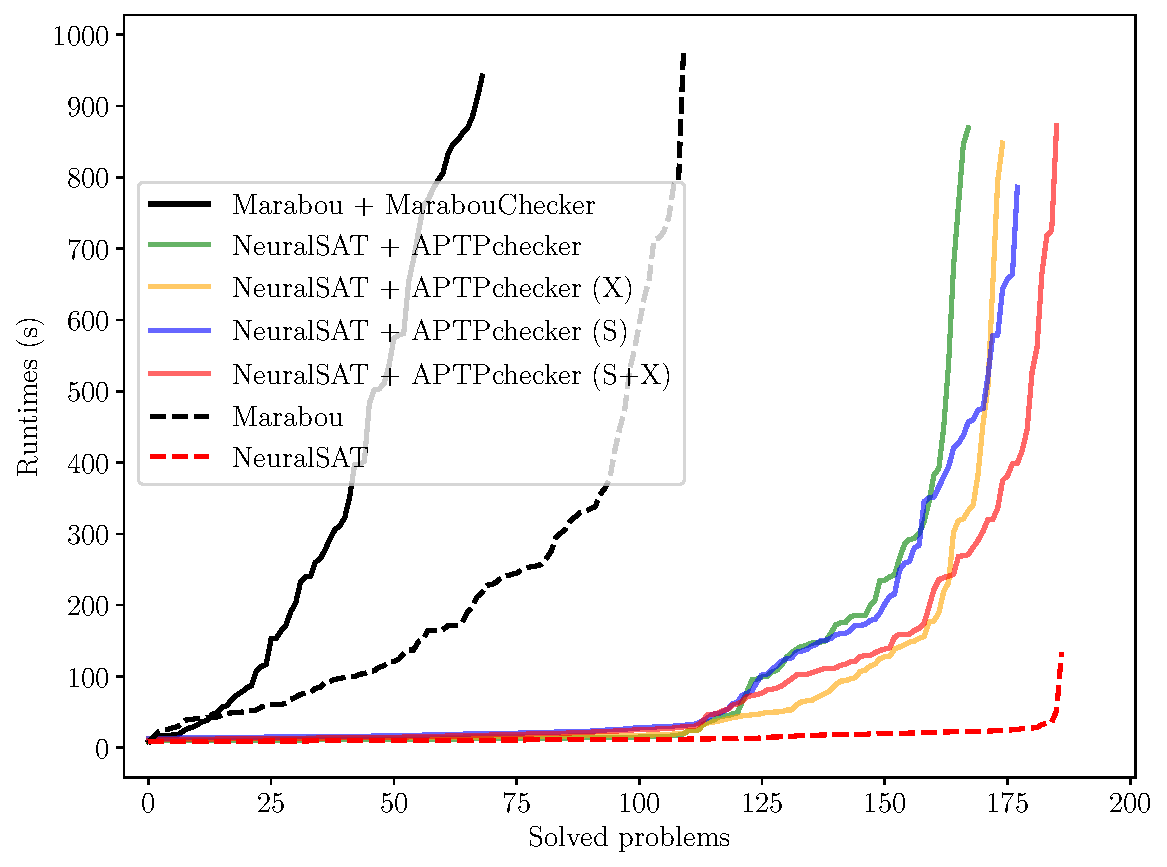
\includegraphics[width=\linewidth]{figure/fnn.pdf}
    \end{minipage}
    \begin{minipage}[t]{0.4\textwidth}
        \centering  
        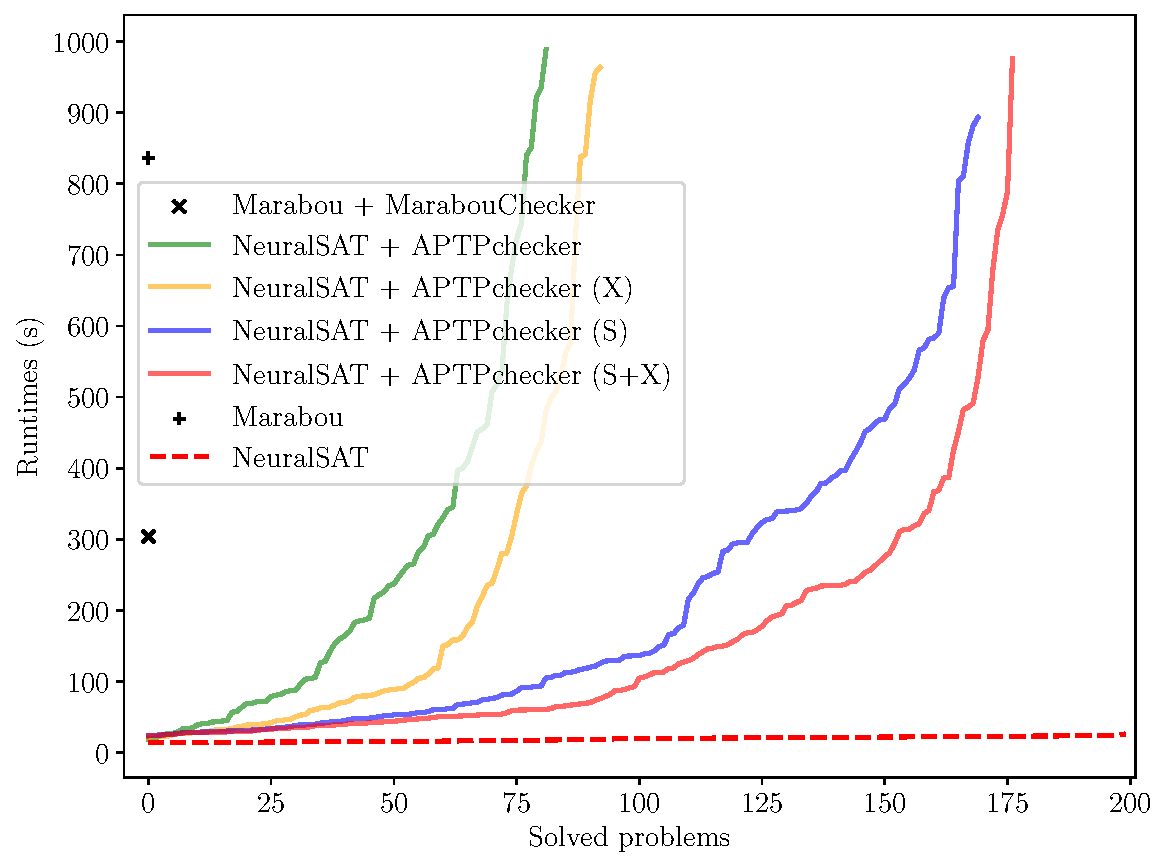
\includegraphics[width=\linewidth]{figure/cnn.pdf}
    \end{minipage}

    % \begin{minipage}[t]{0.45\textwidth}
    %     \centering  
    %     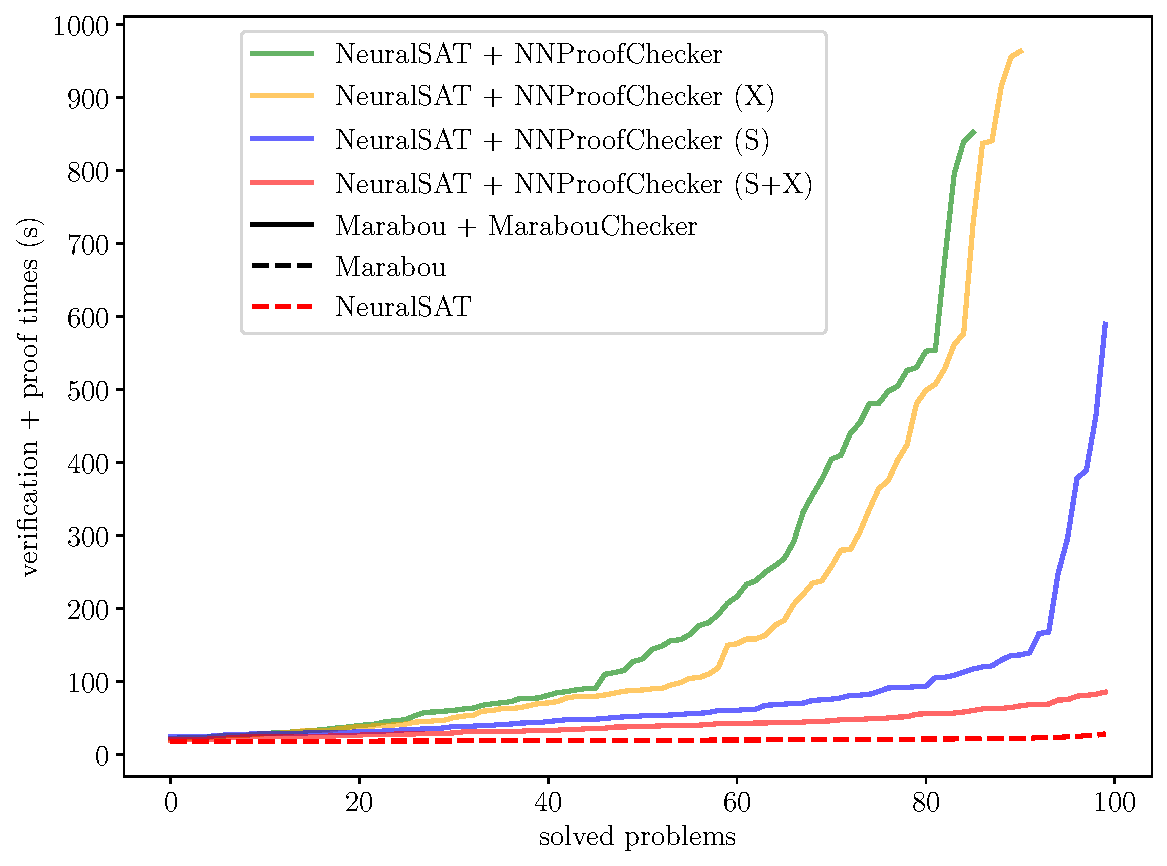
\includegraphics[width=\linewidth]{figure/MNIST_CNN_SMALL.pdf}
    % \end{minipage}
    % \hfill
    % \begin{minipage}[t]{0.45\textwidth}
    %     \centering  
    %     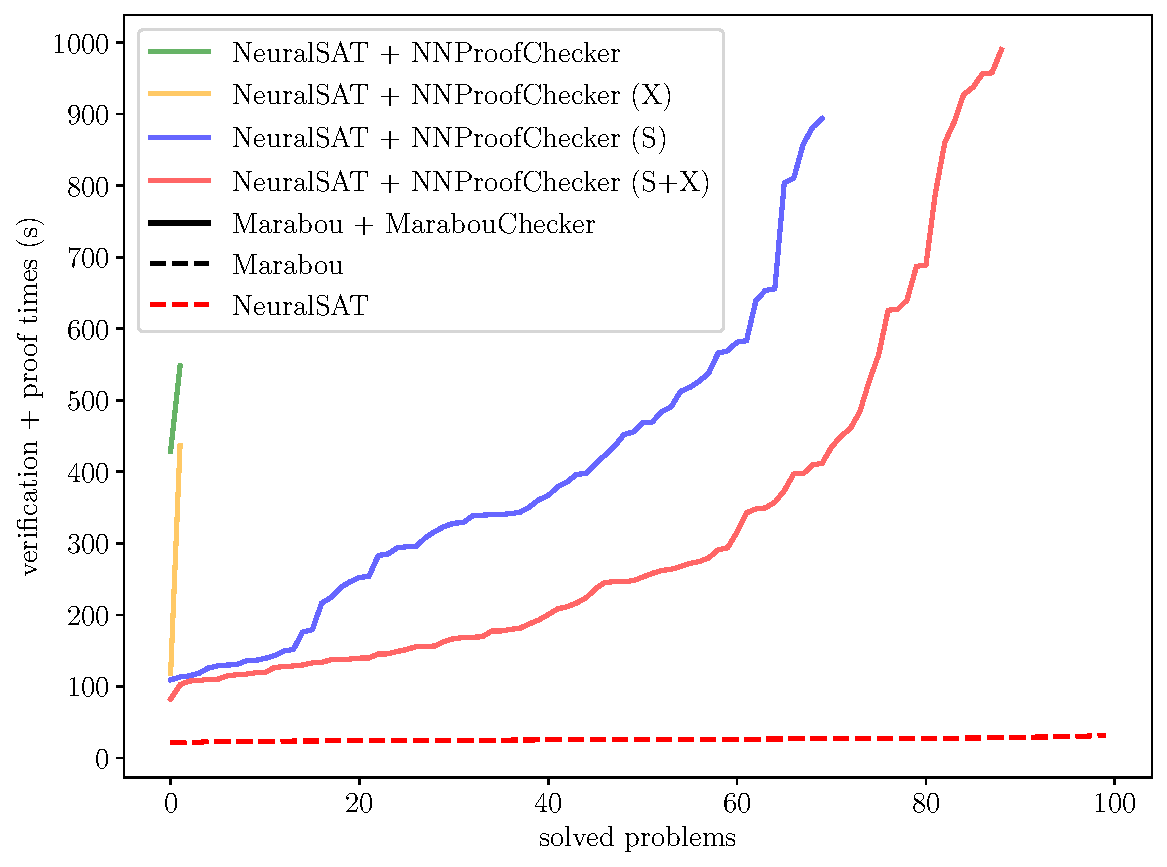
\includegraphics[width=\linewidth]{figure/MNIST_CNN_MEDIUM.pdf}
    % \end{minipage}
    \caption{Cactus-plots for verifiers and proof checkers of FNN (top) and CNN (bottom) benchmarks.}
    \label{fig:cactus-plots}
\end{figure}
\paragraph{Treatments}
RQ1 compares the best performing versions of \marabou{}'s proof checker and \nnproofchecker{}.
For RQ2, we consider two of the three optimizations
implemented in \nnproofchecker{} : proof tree pruning (X), and 
proof stabilization (S).  We kept a third optimization that controls the
degree of parallelization in proof checking fixed at a value of 64 to mitigate
experimental cost; since the independence of sub-proofs means that
proof checking is amenable to linear speedup we felt this aspect of experimentation
was less valuable.
For RQ3, we use both \neuralsat{} and \crown{} to generate proofs; this
constitutes a treatment for this research question as it varies the
verification algorithm.
For each verifier, we explore a base version of the verifier and an optimization:
the stabilization optimization for \neuralsat{} and replacing
the default branch-and-bound decision heuristic with the BaBSR~\cite{bunel2020branch} heuristic
in \crown{}.

\paragraph{Metrics}
In the verification community there are two metrics commonly used to
assess performance: time to solve the problems and number of problems solved
from a benchmark.  We report them both here.

For each \nnproofchecker{} problem we record:
the time to verify that the problem is UNSAT, the time to generate a proof,
the time for \nnproofchecker{} to finish.
If the sum of these for a problem is less than a specified timeout,
1000 seconds in our evaluation, then we say the problem is ``solved''.
For verifiers run alone, a problem is solved if the verification completes
within the timeout.

For each benchmark, we provide cactus plots which plot the time for a problem on the y-axis, and the number of problems solved on the x-axis; problems are sorted on the x-axis from least to largest.
As shown in~\autoref{fig:cactus-plots}, these plots allow one to observe both the time difference between baselines and treatments (vertical distance between lines at a point on the x-axis) and the ability of techniques to solve problems (the maximum x-coordinate for a given line).

We also report the size of proof trees that are generated in \nnproofformat{}.
In the absence of optimizations this defines the \textit{number of sub-proofs}
that need to be checked, but with optimizations the number of sub-proofs may
be reduced, e.g., when an interior node in the tree can be proven.
The complexity of  sub-proofs
may vary significantly, so to provide a more detailed characterization we
also report \textit{MILP complexity}.  \autoref{eq:mip} defines the general form
of each MILP problem, but the problems will vary based on how many of the $a$ variables
defined in \autoref{eq:mip}(d) have a fixed value -- either 0 or 1.   When this
happens the constraint in \autoref{eq:mip}(e) are simplified.
Consequently, we measure MILP complexity as the number of neurons that do \textit{not}
have a fixed value, i.e., the number of unstable neurons.  
\ignore{This does not account for the contribution of \autoref{eq:mip}a,b which is directly
related to network size and input/output dimension.   Is there any way to measure that?}
% \hd{I see. It seems hard since "a"s and constraints do not have the same unit.}

\paragraph{Experimental Setup}
All experiments were run on a Linux machine with an AMD Threadripper 64-core 4.2GHZ CPU, 128GB RAM, and an NVIDIA GeForce RTX 4090 GPU with 24 GB VRAM. 
We used a timeout of 1000 seconds for the combined time of running the verifier,
generating the proof, and then checking that proof.

\subsection{RQ1 : Proof Checking Performance}
\label{sec:rq1}
\autoref{fig:cactus-plots} presents data on the performance
of \nnproofchecker{} relative to both an underlying verifier, \neuralsat{}, and prior work on neural network proof checking, \marabou{}'s proof checker.  
In cactus plots like this, lines that extend further on the x-axis
are better -- more problems solved -- and lines that are lower are better -- faster solve times.
Another way to view these is to pick a point on the x-axis where the plots for two techniques are defined and think of the areas under the two curves as the ``total cost'' to solve that number of problems.
The dashed lines in the plots show the performance of the verifier and the solid lines show the performance of the verifier, proof generation, and the proof checker.  Several configurations of
\nnproofchecker{} are shown, but in this RQ we draw the readers attention
to the plots for the \nnproofchecker{}(S+X) configurations; the rest are discussed in detail below.

The cactus plot for the FNN benchmark (top)
shows that \marabou{} and its checker are able to solve 69 problems or 35\% of the benchmark, whereas \nnproofchecker{} can solve 186 or 93\%.  
For the CNN benchmark (bottom) \marabou{} and its checker can solve a single benchmark, whereas \nnproofchecker{} can solve 177 problems or 89\%.
In total, \nnproofchecker{} solved 363 problems or 91\%, whereas \marabou{}  solved 70 problems or 18\% of all instances.

\begin{figure*}[t]
\begin{subfigure}{0.4\linewidth}
    \centering
    % 
    \begin{minipage}[t]{0.75\textwidth}
        \centering  
        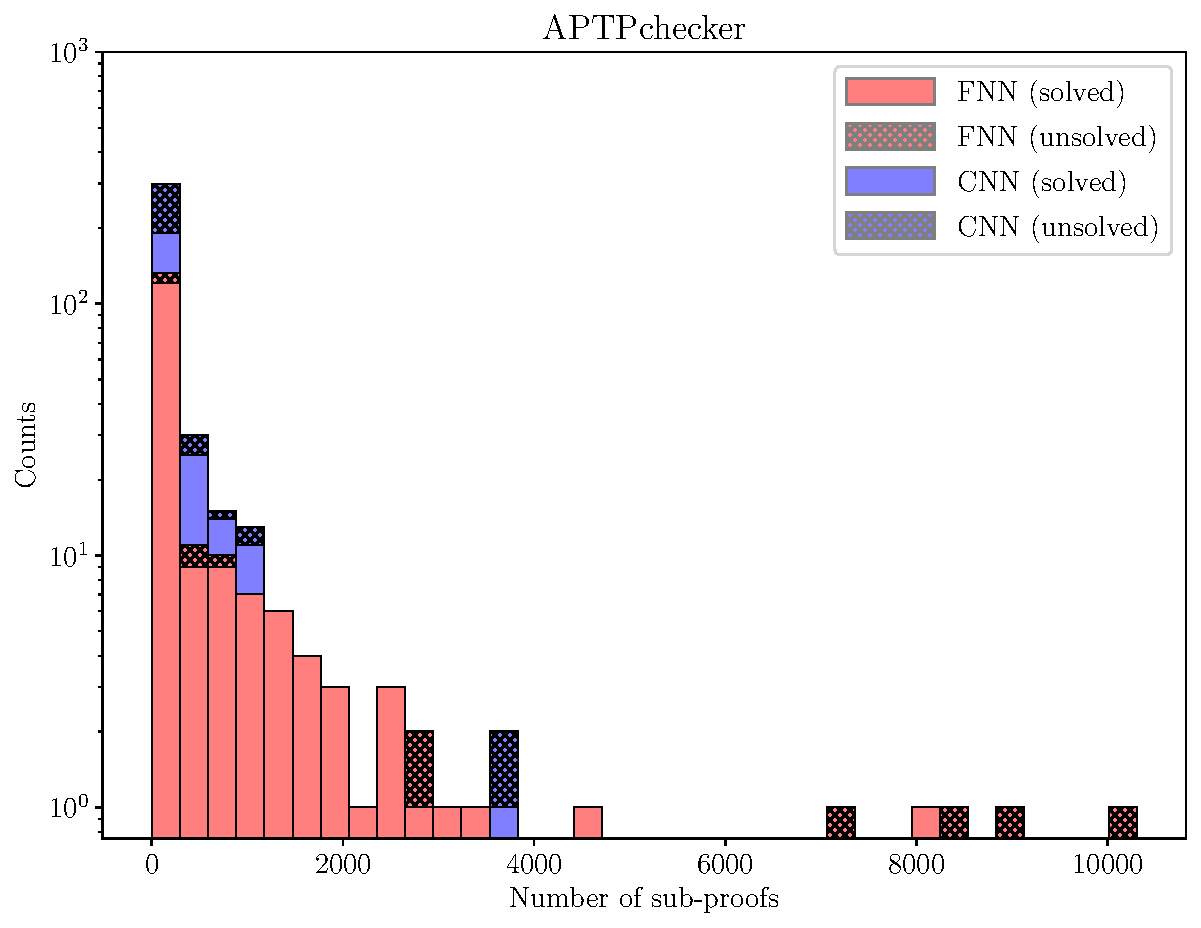
\includegraphics[width=\linewidth]{figure/SUB_PROOFS_NONE.pdf}
    \end{minipage}
    %
    \begin{minipage}[t]{0.235\textwidth}
        \centering  
        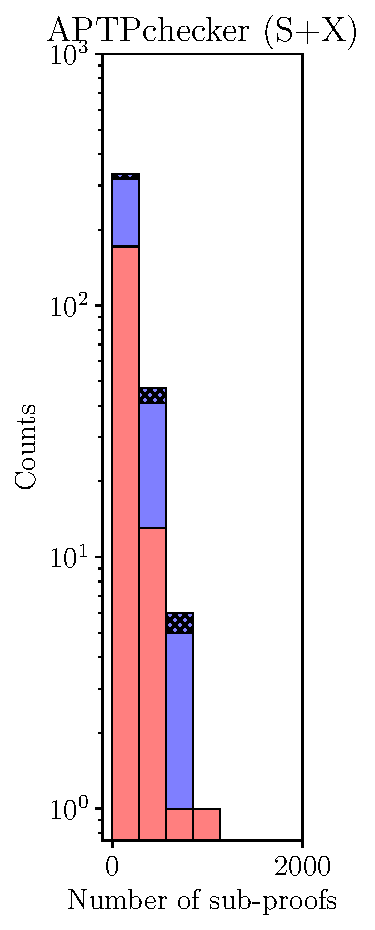
\includegraphics[width=\linewidth]{figure/SUB_PROOFS_SX.pdf}
    \end{minipage}
    \caption{Number of sub-proofs per problem with (right) and without (left) \nnproofchecker{} optimizations.}
    \label{fig:sub-proofs-plots}
\end{subfigure}
\hfill
\begin{subfigure}{0.59\linewidth}
    \centering 
    %
    \begin{minipage}[t]{0.5\textwidth}
        \centering  
        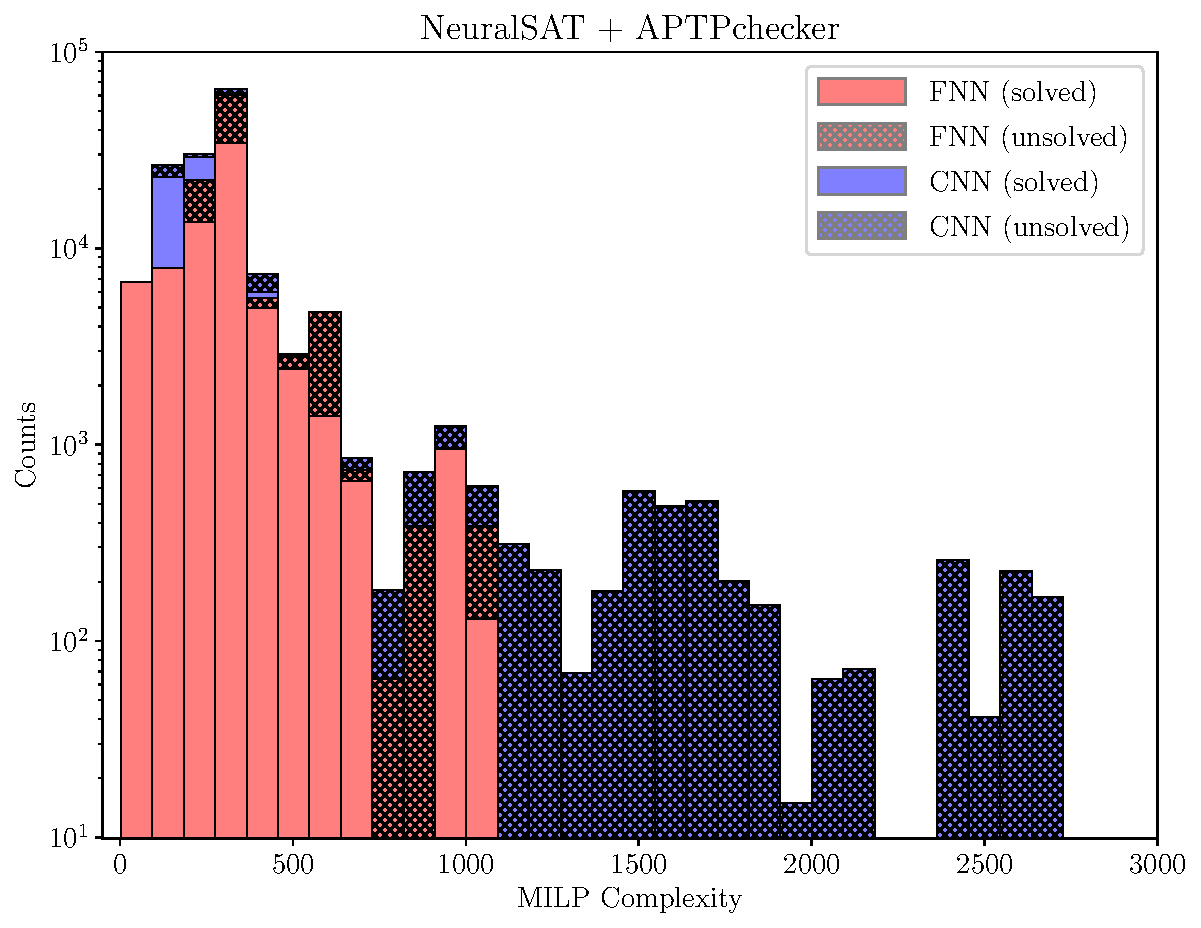
\includegraphics[width=\linewidth]{figure/MILP_COMPLEXITY_NONE.pdf}
    \end{minipage}%
    \begin{minipage}[t]{0.5\textwidth}
        \centering  
        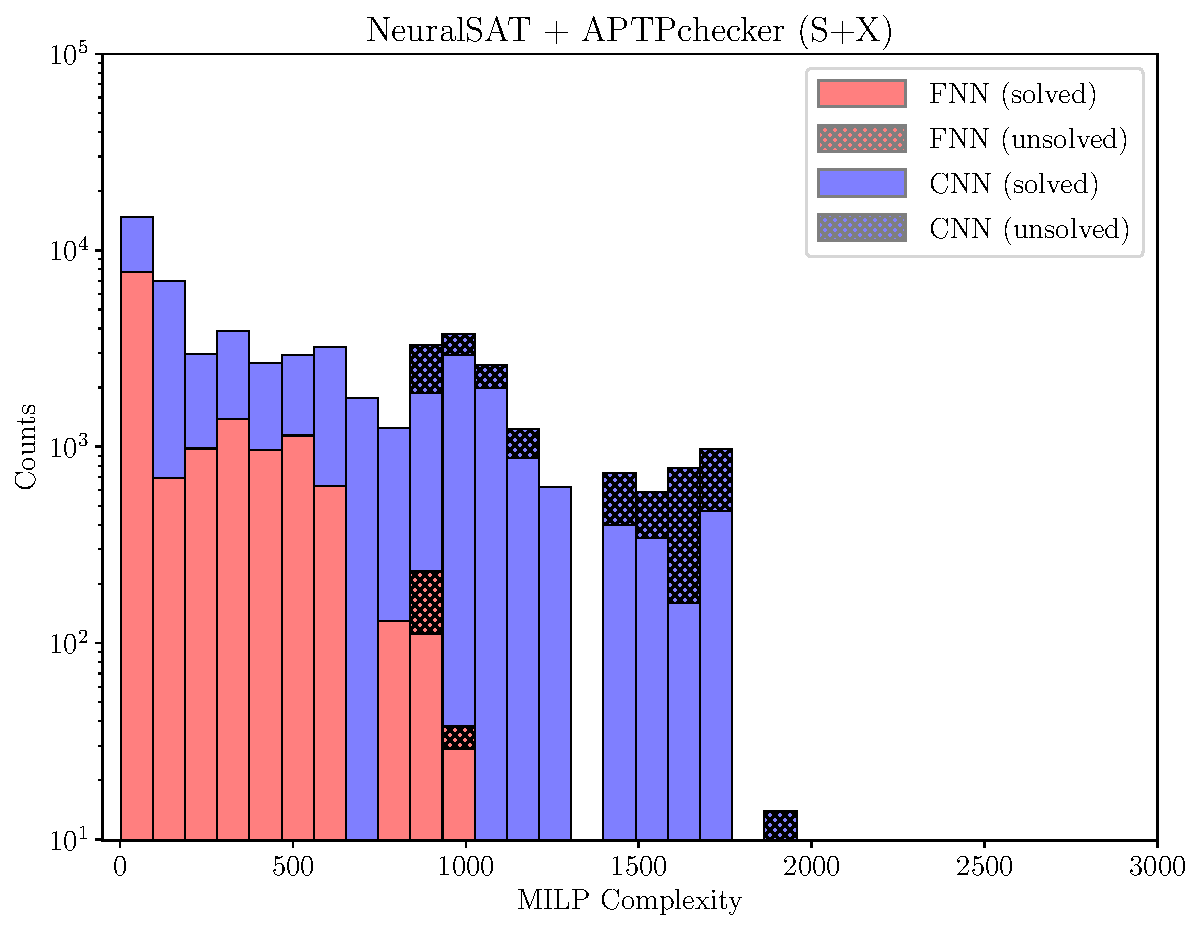
\includegraphics[width=\linewidth]{figure/MILP_COMPLEXITY_SX.pdf}
    \end{minipage}

    \caption{Number of constraints of a given complexity per problem with (right) and without (left) \nnproofchecker{} optimizations.}
    \label{fig:constrs-proofs-plots}
\end{subfigure}
\caption{Data on proof size and complexity.   Y-axes are log-scale due to the range of values.}
\end{figure*}

% \matt{Some of the line number references are no longer resolving below.}
The shape of these cactus plots indicates a high-degree of variability in the cost of proof
checking relative to verification.
From~\autoref{fig:algorithm} it is clear that both the number of leaves in the tree
structure,~\autoref{line:get_leaf}, and the complexity of the model to be checked,~\autoref{line:proof_check_objective1}, are factors that contribute to the cost of proof checking.
To explore those factors we plot their variation across the benchmarks when running \nnproofchecker{}.

\autoref{fig:sub-proofs-plots} (left) plots a histogram of the number of sub-proofs solved per verification 
problem, i.e., the number of nodes of the proof tree.
When interpreting these plots, understand that the y-axis log scale means that vertical
distances have a different meaning as you move upward in the plot.
While the vast majority of the verification problems have proof trees of fewer then 2000 leaves, but 17 of them have larger trees up to a maximum of more than 10000 leaves.
Note also that even among the smaller sized proof trees, there are some problems that cannot be solved.
This is due to complexity of solving the MILP constraints at the leaves of those proof trees.

\autoref{fig:constrs-proofs-plots} (top) plots a histogram of the number of occurrences of MILP problems of
a given complexity across the benchmarks.  Here again we see a spread in data, but unlike with the number of sub-proofs the CNN benchmarks seem to have consistently larger constraints and there is a clear bias among the unsolved problems towards larger constraint size.
To optimize proof checking, we must address both of these sources of complexity.

\begin{tcolorbox}[left=1pt,right=1pt,top=1pt,bottom=1pt]
\textbf{RQ1 Findings}: Proof checking performance varies with both the size of the proof tree and the complexity of the MILP problems at the nodes of the tree.  \nnproofchecker{} can solve 91\% of the problems across the benchmarks and improves on prior work which can solve less than 18\%.
% \tvn{are these numbers correct?  the 2nd paragraph of RQ1 says prior work can do 24\% and \nnproofchecker{} can do 92\%}
\end{tcolorbox}

\subsection{RQ2 : Proof Checking Optimizations}
\label{sec:rq2}
The performance cactus plots~\autoref{fig:cactus-plots} present an ablation
study of the 
pruning (X) and stabilization (S) optimizations of \nnproofchecker{}.
The trend across both benchmarks is consistent with pruning (yellow) and stabilization (blue)
 improving the number of problems solved by 5\% and 36\%, respectively, over the unoptimized
\nnproofchecker{} (green).
The combination of optimizations (red) improves the number of solved problems by 46\%, which is more than the sum of their individual improvements demonstrating that the methods create opportunities for one another for further optimization.
\ignore{
- neither X nor S: 168 (F) + 88 (C) = 256
- X: 175 (F) + 93 (C) = 268
- S: 178 (F) + 170 (C) = 348
}

The \autoref{fig:sub-proofs-plots} (right) and \autoref{fig:constrs-proofs-plots} (right) explore the impact of the S and X optimizations on the number of sub-proofs and MILP complexity.  Across the benchmarks optimizations reduce 
the number of sub-proofs is to less than 1000 and
MILP complexity to less than 2000.   
The reduction in sub-proofs directly contributes to the increase
in performance of \nnproofchecker{}, but the reduction in
MILP complexity is more subtle.   
Integer programming, and thus MILP, is known to be
NP-Hard in general~\cite{garey1979computers}.
The stabilization optimization addresses this complexity by
calculating sets of variables that are forced to take on specific
values based on other constraints in the MILP problem.  For each
such variable, the constraints associated with it is effectively
eliminated.  We can observe this in comparing the left and
right of \autoref{fig:constrs-proofs-plots} where we see both
constraints of higher complexity eliminated and the peak of
the constraint distribution shifted downward from 400 to 100
constraints.  

\ignore{
Sub-problem size
- without S+X:
    + mean: 388
    + std: 1062
- with S+X
    + mean: 142
    + std: 152

MILP complexity
- without S+X: 
    + mean: 329
    + std: 274
- with S+X
    + mean: 493
    + std 449

We performed an analysis of the relationship between size of constraints and number of sub-proofs and determined that these factors are not strongly correlated.
For example, there is a 1 layer CNN model with 27k parameters whose verification
generates 680 sub-proofs where the complexity of the constraints in that proof are at most 109. 
On the other end of the spectrum, verification of a 2 layer CNN model with 180k parameters only requires 81 sub-proofs, but those proofs consist of constraints with complexity of at least 1721.
}

\begin{tcolorbox}[left=1pt,right=1pt,top=1pt,bottom=1pt]
\textbf{RQ2 Findings}: The \nnproofchecker{} optimizations each independently increase the number of proofs that can be checked and in combination they allow
an additional 46\% of the proofs in the benchmarks to be checked.
\end{tcolorbox}

\subsection{RQ3 : Proof Checking and Verifier Optimizations}
\label{sec:rq3}
\autoref{fig:algvariation} shows cactus-plots for two configurations of \neuralsat{} and \crown{} generated proofs across the benchmarks.   The performance of the verifiers, dashed lines, differ across configurations and they are able to 
verify between 337 and 400 problems in the benchmark.
\ignore{Number of Verified/Proved problems
    + abcrown(babsr):   337/335 = 99.4%
    + abcrown:          368/366 = 99.4%
    + neuralsat(SX):    387/363 = 93.7%
    + neuralsat(S)(SX): 400/384 = 96%
}
For both of the verifiers and configurations,
\nnproofchecker{} is able to check between 93.7\% and 99.4\% of the proofs that are generated.
This demonstrates that the \nnproofformat{} is able to encode proofs
generated by differing neural network verification algorithms, and
that \nnproofchecker{} can check them.

% \autoref{tab:sizestats}.
\begin{figure}[t]
    \centering
    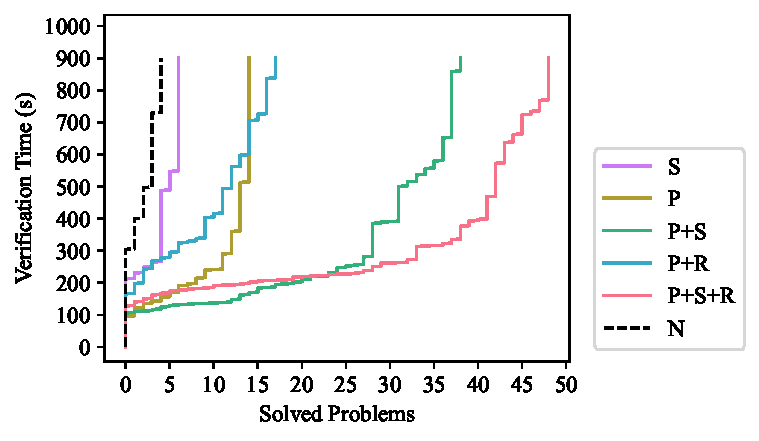
\includegraphics[width=0.8\linewidth]{figure/ablation.pdf}
    \caption{\nnproofchecker{} performance with different verification algorithms.}
    \label{fig:algvariation}
\end{figure}

\begin{table}[t]
    \caption{Proof statistics for best verifier configurations.}
    \label{tab:sizestats}
    \centering
    \begin{tabular}{c|cc|cc}
        \toprule
         \multirow{2}{*}{\textbf{Verifier}} & \multicolumn{2}{c}{\textbf{Num. Sub-Proofs}} & \multicolumn{2}{|c}{\textbf{MILP Complexity}}\\
         & Mean & Median & Mean & Median \\ 
         \midrule
         \neuralsat{}(S) & 95 & 36 & 601 & 545 \\ 
         \midrule
         \crown{} & 230 & 180 & 414 & 179\\
         \bottomrule
    \end{tabular}
\end{table}

We performed an analysis of both the number of sub-proofs and MILP complexity for the proofs generated by the two best performing verifier
configurations.  These values follow a skewed
distribution, so we report the mean and median values in \autoref{tab:sizestats}.   One can observe variation in the
structure of the proofs generated by these verifiers.
\neuralsat{} generates smaller proof trees, but where the
MILP problems are more complex.
In contrast, \crown{} generates significantly larger proof trees,
but with less complex MILP problems.
This variation suggests potential avenues for future work, especially,
when proof checking is important.

For example, \neuralsat{} might include an option to generate larger proof trees, but with smaller MILP problems.  Such proofs would then
be amenable to higher-degrees of parallel solving and mitigate the 
performance bottleneck presented by MILP solver implementations.
One might even consider strategies that use fast verification 
options during development and then when all properties are proven, shift to slower verification options that are more amenable to proof checking.

\ignore{
1. Longer verification time means proof tree will be larger since verifier has to explore larger space
2. If an instance is verified by \crown{}, it will likely be proved by \nnproofchecker{}. In other words, most of timeout instances are due to \crown{} cannot verify (1st phase).

- MILP complexity:
    + neuralsat(S)(SX)  : mean=601.36, std=475.88, median=545.00, min=3, max=1944
    + neuralsat(SX)     : mean=492.40, std=448.81, median=342.00, min=2, max=1956
    + abcrown           : mean=414.35, std=447.02, median=179.00, min=0, max=1957
    + abcrown(babsr)    : mean=409.00, std=448.89, median=166.00, min=0, max=1952

They share the same MILP base model since their base models are all generated from SX setting.
neuralsat(S)(SX) has larger MILP complexity in average means that its proof trees are often shallower than others. In other words, neuralsat(S) explores smaller space than others -- which is true.

- number of sub proofs:
    + neuralsat(S)(SX): mean=95.11,   std=117.13, median=36.00,  min=0, max=829
    + neuralsat(SX)   : mean=142.00,  std=151.72, median=106.00, min=1, max=1132
    + abcrown         : mean=229.96,  std=199.23, median=180.00, min=0, max=1152
    + abcrown(babsr)  : mean=228.10,  std=170.88, median=188.00, min=0, max=857

- Number of leaves:
    + neuralsat(S)(SX): mean=236.59,   std=447.80,   median=37.50,  min=0, max=3627
    + neuralsat(SX)   : mean=902.25,   std=4957.22,  median=219.00, min=6, max=91318
    + abcrown         : mean=3007.42,  std=12742.09, median=561.00, min=0, max=138918
    + abcrown(babsr)  : mean=11714.62, std=41909.72, median=781.50, min=0, max=509765
}


\begin{tcolorbox}[left=1pt,right=1pt,top=1pt,bottom=1pt]
\textbf{RQ3 Findings}: \nnproofformat{} is robust to variation in different verification algorithms and \nnproofchecker{} is applicable to any such proof and effective in checking
the vast majority of those arising from the benchmarks.
\end{tcolorbox}



\chapter{Conclusion}

\appendix
\chapter{Logics and Linear Programming}\label{app:logics}

\section{Logics and Satisfiability}\label{app:logics}
\section{Linear Programming}\label{app:lp}

\tvn{Hai, give some LP background here.}

\bibliographystyle{abbrv}
\bibliography{book.bib}

\appendix

\end{document}
